\documentclass[pageno]{jpaper}
%\usepackage{latex8}

% \usepackage[margin=1in]{geometry}
\usepackage{amsmath,amsthm,amssymb}
\usepackage{enumerate}
\usepackage{bbold}
\usepackage{graphicx}
\usepackage{multirow}
\usepackage{hhline}
\usepackage{color}
\usepackage{tsgcomments}

%******************************************************************************
% Anonymization Macros
% Usage : \ifanonymized{anonymized}{notanonymized}
% Uncomment one of the following

\newcommand{\ifanonymized}[2]{#1} % Anonymized
% \newcommand{\ifanonymized}[2]{#2} % Not Anonymized
%******************************************************************************

% Space optimization. cut lower priority first.
% low priority: nice to have, but does not really affect the content
\newcommand{\loptional}[1]{#1} 

% high priority: good content to have, but not critical
\newcommand{\hoptional}[1]{#1} 


\pagestyle{empty}

\setlength{\pdfpagewidth}{8.5in}
\setlength{\pdfpageheight}{11in}

\begin{document}

\title{
\vspace{-0.1in}
    Timing Compartments: An Architecture Abstraction for Timing Isolation
}

\ifanonymized{
    \author{}
}{
    \author{
    Andrew Ferraiuolo, Yao Wang, and G. Edward Suh\thanks{The first two authors 
    contributed equally to this work.}\\
    Cornell University\\
    Ithaca, NY 14850, USA\\
    \{af433,yw438,gs272\}@cornell.edu
    }
}


\date{}
\maketitle

\thispagestyle{empty}

\begin{abstract}
    This paper presents timing compartments, a hardware architecture primitive 
    that eliminates microarchitectural timing channels between groups of 
    processes or VMs. Timing channels violate the boundaries between these 
    software system entities despite conventional security techniques such as 
    access controls and virtual memory. Unlike other covert/side channels such 
    as power monitoring timing channels can be exploited in software without 
    physical access to the device. 
%    When coupled with conventional security 
%    techniques, timing compartments enable distrusting entities to share 
%    hardware with a level of assurance that is comparable to executing
%    on separate hardware. By separating timing channel control from control for 
%    explicit communication channels, timing compartments afford the flexibility 
%    to pay for timing channel protection only when necessary. 
    To realize timing 
    compartments, we design and experimentally evaluate a full multi-core 
    processor that eliminates timing channels for critical shared hardware 
    components. 
    In particular, we identified new sources of timing channels including
    cache coherence mechanisms and module interfaces, and provide solutions for them.
    The experimental results suggest that the overheads of
    timing compartments can be rather low in modern microprocessors, especially 
    when the number of timing compartments is small.

\end{abstract}

\section{Introduction}

Timing channel attacks are becoming a major threat as hardware is increasingly 
consolidated and shared by distrusting entities, which traditionally have been
isolated on their own physical machines. For example, in cloud computing, mutually distrusting 
parties own virtual machines on shared hardware. In mobile devices, users often
run downloaded applications that cannot be trusted to handle private personal
information.
While untrusted applications can be sandboxed using
traditional access control mechanisms to limit explicit communications,
timing 
channels can still be used by a malicious program to extract or leak secrets.
%from other co-located applications.
Further, unlike physical side-channel attacks such as power analysis that require
physical proximity, timing channels can be exploited in software by remote
adversaries.

%For example, end users download untrusted 
%applications from the Internet which can then execute on the same hardware as 
%software that will handle the user's sensitive financial data. System on chip 
%platforms tightly integrate hardware designed by directly competing companies.  
%This necessitates hardware sharing among the drivers and proprietary algorithms 
%owned by these distrusting companies. 
%So timing channels 
%vulnerabilities are not only prevalent, but easy to exploit.

%Many of the systems that are vulnerable to timing channels do take security 
%measures to prevent explicit channel attacks. In a cloud platform, the 
%hypervisor performs physical address translation on behalf of the virtual 
%machines to isolate the virtual machines in the physical memory. Hypervisors 
%also use access controls to isolate virtual machines, typically relying on 
%hardware abstractions such as protection rings. However, these security 
%mechanisms are not enough. They do nothing to prevent coresident VMs from 
%leaking secret information through timing channels induced by hardware sharing.

In this paper, we investigate an architecture abstraction, named timing compartments (TCs),
which allows software to explicitly request strong timing isolation among software
entities that share a multi-core processor.
The goal of timing compartments is to remove fine-grained microarchitecture-level timing interference
that cannot be controlled in software and thus enable strong timing isolation that is
comparable to running a software entity on its own processor.
The timing compartment is designed to prevent both unintentional information leaks
through side channels and intentional leaks through covert channels.
%Using the timing compartments, software designers can specify a timing protection
%requirement that is necessary for each application. 
%More importantly, 
When coupled with software-level protection mechanisms to control timing channels 
through coarse-grained events such as scheduling and I/O, timing compartments
can enable comprehensive timing isolation of program or a virtual machine.

The timing compartment is designed so that timing isolation can be
separated from traditional access control. For example, multiple programs or
virtual machines that are isolated from each other using virtual memory may
be grouped into a single timing compartment if they either belong to the 
same trust domain or do not require timing channel protection. 
This separation provides a system the flexibility to only pay overhead for
timing channel protection when it is truly necessary.

To realize the timing compartments, a multi-core processor needs to be
re-designed to control inter-core timing interference in shared hardware
resources that cannot be efficiently controlled in software.
In this paper, we identify major resources that can be shared concurrently among
multiple cores on a typical multi-core processor, namely shared caches,
on-chip interconnect, cache coherence mechanisms, and off-chip memory controllers,
and augment each shared resource with a mechanism
to eliminate timing interference.

This ``full-processor'' protection study revealed new sources timing
channels on a multi-core processor that have not been studied yet.
For example, we found that interfaces between hardware modules and 
a cache coherence mechanism can lead to timing channels, and demonstrate
a covert channel attack using the coherence traffic interference.
The integration effort also showed that protection mechanisms need to
be carefully coordinated in order to avoid unnecessary inefficiencies.
To the best of our knowledge, this paper represents the first study
that implements comprehensive timing channel protection for a full 
multi-core microprocessor and evaluates the overhead.

%Recent studies have investigated mechanisms to prevent
%timing channels in various microarchitecture components, including
%shared caches \cite{icache,newcache,deconstructing,cachegames}, processor pipelines 
%\cite{pipelines}, branch predictors~\cite{branchpred,predictingbranch}, on chip 
%networks~\cite{yaonocs}, and memory controllers~\cite{ushpca14}.
%However, we found that the full timing channel protection for a multi-core
%processor requires more than simply integrating previous protection 
%mechanisms. Our study identified new sources of timing channels at
%interfaces between hardware modules and also found that protection
%mechanisms need to be coordinated together to avoid unnecessary inefficiencies.

%Ascend~\cite{ascend} considers external timing 
%channel attacks, but does not prevent timing channels due to shared resources.  
%Execution leases~\cite{execution_leases} provide an architecture abstraction
%that prevents external timing channels by bounding the execution time of a code 
%segment, but Execution leases do not prevent the internal timing channels 
%caused by shared hardware. GLIFT \cite{citation_needed} can be used to identify 
%timing channels, but does not prevent them. Further, the area, power, and 
%performance overheads are prohibitively large.

%Unlike previous work, timing compartments eliminate all internal timing 
%channels in a conventional microarchitecture. When combined with standard 
%access controls, timing compartments achieve the security of running mutually 
%distrusting software on separate hardware with some of the performance benefits 
%of sharing hardware. To the best of our knowledge, this is the first 
%architecture technique to reach this goal. This work is also the first to 
%experimentally evaluate the cost of applying timing channel protection to every 
%vulnerable component. Further, we show that integrating these protection 
%mechanisms to form a complete system with minimal performance overheads is 
%nontrivial and requires careful coordination. In the process of designing an 
%integrated timing channel protection system we identified two novel 
%microarchitectural timing channels. In addition to these contributions we 
%extend the taxonomy of timing channels and show how this taxonomy can be used 
%to identify techniques that can eliminate timing channels in any additional 
%components (e.g. accelerators).

The simulation results suggest that the performance overhead of supporting
timing compartments is relatively low, especially when the number of timing
compartments that simultaneously run is small.
%for the SPEC benchmarks. 
Even though
the timing compartments require shared resources to be statically 
allocated, the overall impact on the performance is limited by the fact
that the protection only affects infrequent cache misses and that modern
processors include large caches. 

The following summarizes the main contributions.

\begin{itemize}
\item The paper introduces a new abstraction that enables software to
explicitly remove microarchitecture-level timing interference on a multi-core.
%The timing compartment enables new
%applications that require strong timing isolation of software modules.
\item The paper identifies new timing channels on a multi-core processor,
including the one through cache coherence, and presents
comprehensive protection mechanisms for a full multi-core processor.
\item The paper shows how protection mechanisms need to be coordinated to
reduce the overhead.% of timing compartments.
\item The paper evaluates the performance overhead of the full-processor
timing channel protection, and shows that the overhead can be reasonable.
\end{itemize}

The rest of the paper is organized as follows.
Section 2 introduces timing compartments and 
presents example applications that can be enabled by strong timing isolation.
Section 3 identifies the sources of timing channels in a multi-core processor, and
describes protection mechanisms to eliminate them. 
Section 4 presents how the hardware protection mechanisms based on time-division
multiplexing need to be coordinated to reduce overhead.
Section 5 evaluates the proposed architecture. Section 6 discusses related
work, and Section 7 concludes the paper.

\section{Timing Compartments}
    Timing compartments are a new architecture primitive that control timing 
    channel leakage among software entities that share hardware. When combined 
    with explicit channel protection (such as access controls) timing 
    compartments provide total software isolation.
    A timing compartment consists of one or more software entities. Here a 
    software entitiy is some system abstraction (such as processes or threads 
    in a single OS system or virtual machines in a virtualization based system) 
    that execute software and have an owner.
    
    Timing channels between timing compartments must be controlled according to 
    a policy that meets the security requirements of the system. This policy 
    entails of a lattice of security levels such as $\mathtt{low} \leq
    \mathtt{high}$. A timing compartment can only leak information to a 
    preceeding timing compartment in the lattice. This lattice model is quite 
    expressive. The lattice $\mathtt{low} \leq \mathtt{high}$ defines a policy 
    where a high assurance software entity can not leak information to a low 
    assurance one. The lattice $\mathtt{T_1} \nleq \mathtt{T_2}, \mathtt{T_2} 
    \nleq \mathtt{T_1}$ defines a policy where $T_1$ and $T_2$ are mutually 
    distrusting. By convention, security lables share names with their timing 
    compartments. 
 
    To enforce the policy a trusted software component called the timing 
    compartment manager (TCM) confines software entities into TCs. The TCM then 
    informs the hardware of the TCs and policy. At runtime, the TCM tags 
    hardware requests with a tag to indicate the TC of the software entity that 
    made the request. 

    Timing compartments only address timing channels; they do not control 
    information flow through explicit channels. Handling these concerns 
    separately allows for more flexibility in the overall system design.  When 
    designing a secure system, implementors must consider how the cost required 
    to carry out a particular attack compares with other attacks, the potential 
    damage that could be caused by an attack, and the cost and performance 
    impact of implementing the security mechanisms needed to stop it. This 
    enables timing compartments to provide timing channel protection only to 
    software entities that need it.

    \subsection{Applications}
    This section describes how to apply timing compartments to protect the 
    vulnerable systems described in section \ref{sec:cloud_scenario}.
    \subsubsection{Cloud Computing}
    In the cloud computing system described eariler, VM1 and VM2 are both 
    running applications with high security needs. Both distrust eachother and 
    all other VMs in the system. VM3 and VM4 are running programs that require 
    a lot of performance, but have low security needs. All VMs implicitly trust 
    the hypervisor. Figure \ref{fig:cloud_tcs} shows timing compartments can be 
    applied to meet the needs of this system. VM1 and VM2 are confined to their 
    own timing compartments TC1 and TC2, but VM3 and VM4 are grouped in TC3.  
    The hypervisor is extended with a TCM and confined to TC0 since it also 
    requires timing channel protection. 
    
    \begin{figure}
        \begin{center}
            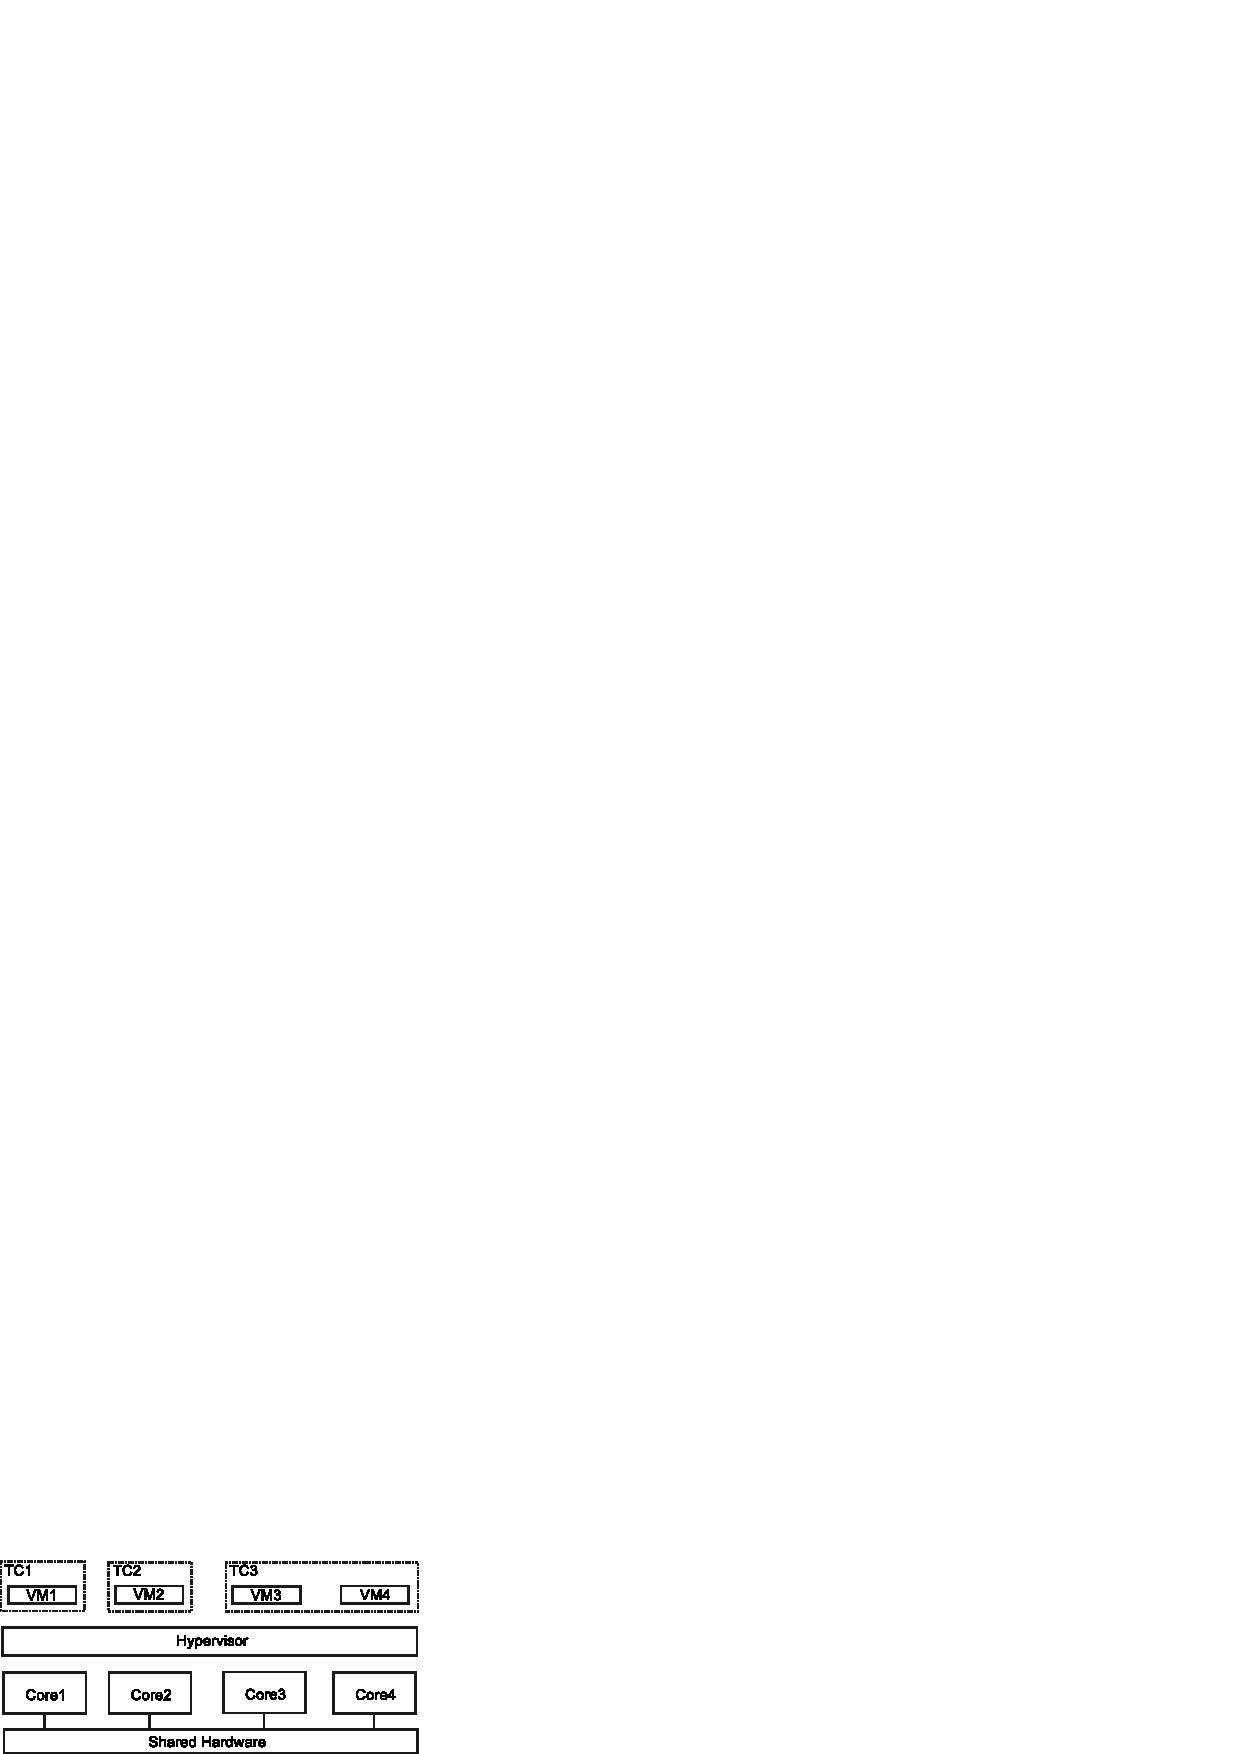
\includegraphics[width=2.1in]{figs/cloud_tcs.pdf}
            \caption{ An application of timing compartments to a cloud 
                computing environment. The hypervisor and high assurance VMs 
                are confined to their own TCs while low assurance VMs share TC3
            }
            \label{fig:cloud_tcs}
        \end{center}
    \end{figure}

    \begin{figure}
        \begin{center}
            \includegraphics[width=1.5in]{figs/cloud_lattice.pdf}
            \caption{ A lattice governing the timing compartments of the cloud 
                computing environment. TC3 preceeds TC1 and TC2. TC1 and TC2 
                are incomparable with each other, but preceed TC0
            }
            \label{fig:cloud_lattice}
        \end{center}
    \end{figure}

    The lattice in Figure \ref{fig:cloud_lattice} defines the policy. TC3 
    preceeds both TC1 and TC2 implying timing channel leakage from VM3 or VM4 
    to any other VM is not controlled. However, VM1 and VM2 cannot leak 
    information to VM3 or VM4. Additionally, VM1 and VM2 cannot leak 
    information to each other since TC1 and TC2 are incomparable. All other TCs 
    preceed TC0, so leakage from any VM to the hypervisor is not controlled, 
    but the hypervisor cannot leak any information to the VMs.This meets the 
    security requirements of VM1 and VM2 since both are totally isolated from 
    the other VMs through timing channels. Since VM3 and VM4 share a timing 
    compartment, they can share resources normally and incur minimal 
    performance overheads.

\section{Microarchitecture-Level Protection}

This section discusses internal timing channels in typical
multi-core processors and mechanisms to control them.

\subsection{Baseline Architecture}

    \begin{figure}
        \begin{center}
            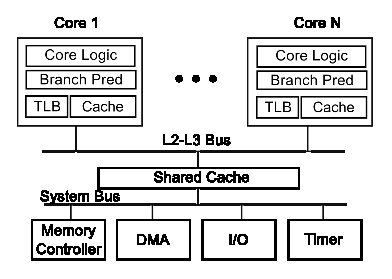
\includegraphics{figs/baseline.eps}
            \caption{Baseline multi-core architecture.}
            \label{fig:baseline}
        \end{center}
    \end{figure}

Figure \ref{fig:baseline} shows a baseline multi-core architecture that we
extend with timing compartments in this paper. The architecture
has multiple cores, each with a core pipeline, a branch predictor, a TLB,
and one or more private caches. 
The cores are connected to a shared cache via an on chip network. A shared system 
bus connects the shared cache to a memory controller that manages requests to 
main memory.
We assume that each core may be time shared by multiple timing
compartments, but only one timing compartment, which we say is active, may run on each core
at a time. This assumption can be relaxed if timing channel protection
is added to per-core resources.

\Ed{Perhaps move all the assumption that we make here?}

%A trusted software layer (such as 
%an operating system) allocates software entities (such as processes) to the 
%cores. 

\subsection{General Protection Approaches}
\label{sec:general_approaches}

Here, we present a classification of internal microarchitectural timing channels 
and a framework of general solutions to address each type.
We follow these approaches to design our
protection mechanisms. These approaches also provide guidelines to
develop new protection mechanisms for components that are not included in
our baseline architecture.

\subsubsection{TCID}

The hardware protection mechanisms track which timing compartment originated 
each request and handle the requests accordingly. Each core has a register that 
stores the timing compartment ID (TCID) of the TC currently active on that core. This is used to derive 
the tags that are appended to requests originating from that core. The TCID is 
$log\ n$ bits where $n$ is the number of cores in the processor.
Events such as network packets or cache accesses that use shared resources are 
tagged with the TCID of the corresponding core. 
The timing channel protection mechanisms use this TCID to distinguish accesses
from among different timing compartments.

\subsubsection{Classification of Internal Timing Channels}

There exists an internal timing channel from one entity (say $E1$)
to another ($E2$) whenever the timing of an action of $E1$ can be affected 
by the behavior of $E2$.

There are two types of such timing channels in hardware: state-based
and contention-based.
A \emph{state-based} timing channel occurs whenever there is a state element 
with an access time that depends on its content and that state element is 
shared among multiple entities.
For example, a conventional shared cache has state-based timing channels, because 
its cache hits are faster than misses.
A \emph{contention based} timing channel occurs whenever multiple entities 
share a resource that can handle only finitely many requests at a time.
Conventional buses have contention-based timing channels.

\subsubsection{State-Based Timing Channel Protection}

%Caches, TLBs, and branch predictors all have state-based timing channels. 
%In 
%each, requests that use an entry that is present in the state elements (e.g.  
%cache hits) are faster than requests to entries not present (e.g. cache 
%misses). The state elements can contain a finite number of entries, so entries 
%must be evicted and replaced with new ones. One software entity can evict 
%entries owned by another, causing interference and timing channel leakage if 
%the choice of entries evicted correlates with a secret. 
In general, the state-based 
timing channels can be removed by applying flattening, partitioning, or 
flushing.
Flattening eliminates the dependence of access time on the state by forcing 
every access to finish in the same (worst case) time. For example, to remove timing 
interference in the row buffers of DRAM, all DRAM accesses may be treated as 
a row buffer miss.
For some components, this is a 
brute-force approach. Applied to caches, every access must be treated as a 
miss, so this is equivalent to removing the cache. 

Partitioning removes interference by ensuring that each entity can
only affect a disjoint subset of state elements. The partitions
should not change dynamically depending on the run-time demands of entities.
In the simplest case, partitions can be static.
However, partitions do not need to be homogeneous and can be sized according 
to static performance characterizations of each software entity (assuming this 
information can be made public and does not depend on secrets).

%prevents software entities that share state elements from 
%interfering. Static partitioning is realized by dividing the state elements 
%into separate partitions for each software entity. Entities are only allowed to 
%evict entries within their own partitions. Partitions must either be static, or 
%at least not resized or moved based on the dynamic behaviour of an entity.
%% If a partition is increased for an entity intensively using the state 
%% elements, the other entities can detect that their partitions have been 
%% resized and information is leaked.
%However, partitions do not need to be heterogeneous and can be sized according 
%to static performance characterizations of each software entity (assuming this 
%information can be made public).

Flushing can remove state-based timing channels for a resource that is time-shared.
For example, a branch prediction table may be cleared on a context switch.
%At the end of a time quantum, the state elements are completely cleared before 
%passing ownership of the state elements to the entity in the next time quantum.  
%Resources that can be flushed can also be partitioned, and there are tradeoffs 
%between these approaches.
% Flushing increases the time wasted at the end of a time quantum if flushing 
% cannot be done in less than one clock cycle. Clearing the state between time 
% quanta also increases the number of slower accesses at the start of the 
% quanta (e.g. it causes more cold cache misses). However, partitioning reduces 
% the total number of state elements that can be allocated to each entity. 
In general, there is a trade-off between partitioning and flushing.
For long time slices (e.g. when context switching is infrequent), 
flushing is preferable because it allows the full capacity to be used by
each timing compartment. In contrast, partitioning may
offer better performance for short time slices by reducing cold misses.
%time to reload
%the state on a context switch.

\subsubsection{Contention-Based Timing Channel Protection}

%Contention based timing channels arise whenever a resource that is shared among 
%multiple software entities can only handle a finite number of requests at a 
%time. 
Contention based timing channels can be removed by duplication or by
time division multiplexing (TDM). Duplication removes interference by
allocating dedicated resources for each timing compartment.
However, this has obvious area overhead implications. If 
duplication is infeasible, time division multiplexing can be used.
%TDM 
%defines a schedule where each software entitiy is guaranteed a period of time, 
%called a time quantum, where only that entity can use the resource. The 
The schedule of time slices must either be static or independent of the 
dynamic behavior of software entities.

%\subsubsection{External Timing Channel Protection}
%
%Though external timing channels are outside the scope of this 
%paper, there are a class of timing channels that are internal to hardware, but 
%appear as external timing channels between two software entities. This form of 
%external timing channel exists in systems where distrusting software entities 
%must communicate. For example, one software entity might be a user space 
%process and another might be a process that performs only high-assurance 
%operations. The user space process requests the high-assurance process to 
%perform some operation on its behalf. The user space process can directly 
%observe the execution time of the other process. This type of timing channel 
%can be solved in software by forcing the observable execution time to 
%equal the worst case execution time, stalling if necessary.


\subsection{Full-Processor Protection}

Timing compartments use hardware mechanisms that control all internal timing 
channels in a microprocessor. Designing a full processor with timing channel
protection may seem rather straightforward. In our baseline architecture, there are
only three main structures that are shared concurrently: a shared cache, on-chip
buses, and a memory controller. Moreover, recent studies have proposed mechanisms
to control timing channels in each of them. For example, researchers have proposed
statically partitioning the shared cache \cite{percival}, and using time division 
multiplexing with a fixed schedule for the on-chip interconnect 
\cite{yaonocs, surfnoc} and the memory controller \cite{ushpca14}.

%Many microarchitectural timing channels and corresponding solutions are 
%well-known. Shared caches create a state-based timing channel where interfering 
%entities cause cache block replacements. This can be prevented by partitioning 
%the cache among the entities. On chip networks and buses have
%timing channels since only one entity can use the bus at a time. Time division 
%multiplexing can resolve this issue \cite{yaonocs}. The authors of 
%\cite{ushpca14} have exposed timing channels in the main memory and memory 
%controller. They propose time division multiplexing the memory controller, 
%partitioning the memory controller queueing structure, and using a closed-page 
%row buffer management policy to close these timing channels. 
%%%%% It isn't totally obvious that private resources are actually shared, and 
%%%%% we don't have a citation for this, so maybe it doesn't need to be here..
% Finally, the private, per-core resources of the system such as the branch 
% predictors, TLBs and private caches also create timing channels since 
% software entities share cores through time multiplexing (for example, 
% processes may be context switched in and out of the same core). These can be 
% resolved by flushing the state elements of these resources on before moving a 
% new software entity onto the core.

However, achieving secure and efficient timing channel protection on a full processor
requires much more than simply putting known protection mechanisms
together. During the design process, we found three new sources of timing channels
in module interfaces that were not discussed previously, and found a bug in the
memory controller protection \cite{ushpca14}.
%The cache protection scheme also needed to be slightly changed to handle cases when timing
%compartments have shared memory pages. 
We also found that time multiplexed
microarchitecture structures must be carefully coordinated in order to avoid 
unnecessarily high overheads. 
%%%%% We have not demonstrated total starvation in practice or on paper.
% or total starvation.

The rest of this section provides a detailed list of timing channels in our
baseline architecture, and presents a protection mechanism that we use for each of them.
Table \ref{table:timing_chan_summary} summarizes these timing channels and
solutions. 
Then, the next section discusses how these protection mechanisms
need to be managed and coordinated together.
We note that the processor design here uses simple static protection
mechanisms that prevent timing channels in both directions. The mechanisms 
can be further optimized for efficiency.

\def\novelcolor{Green}
\begin{table*}
\begin{tabular}{l|l|l|l}
    \hline
    Component & Timing Channel & Classification & Solution\\
    \hline
    \multirow{3}{*}{Shared Caches}
    & Replacement & State  & Set Partitioning \\
    \hhline{~---}
    & {\color{\novelcolor}MSHRs}
    & {\color{\novelcolor}Contention }
    & {\color{\novelcolor}Duplicate MSHR Banks} \\
    \hhline{~---}
    & {\color{\novelcolor}Response Ports}
    & {\color{\novelcolor}Contention }
    & {\color{\novelcolor}Separate Queues \& Time Multiplexing}\\
    \hline
    \multirow{5}{*}{DRAM \& Memory Controller}
    & Page Faults & State  & Address Space Partitioning \\
    \hhline{~---}
    & DRAM Resources & Contention  & Time Multiplexing \\
    \hhline{~---}
    & Queueing Structure & State  & Partitioned Queue \\
    \hhline{~---}
    & Row Buffer & State & Closed Page Policy (Flattening)\\
    \hhline{~---}
    & {\color{\novelcolor} Response Ports} 
    & {\color{\novelcolor} Contention }
    & {\color{\novelcolor} Separate Queues \& Time Multiplexing}\\
    \hline
    \multirow{2}{*}{Network} 
    & Interconnect Contention & Contention & Time Multiplexing \\
    \hhline{~---}
    & Queueing Structure & State & Partitioned Queue \\
\end{tabular}
    \caption{Summary of timing channels and protection approaches. Green represents new timing channels that were not identified in previous work.}
    \label{table:timing_chan_summary}
\end{table*}

\subsection{Shared Caches}
\mbox{}\newline
\textbf{Cache State \& Replacement}
The shared cache causes state-based timing channel vulnerabilities, because accesses
from one timing compartment may evict the cache blocks of another timing compartment.
This state-based timing channel is the focus of prior cache timing channel 
studies.
%to the memory hierarchy for addresses that are stored in the cache (cache hits) 
%are returned faster than requests for entries not stored in the cache (cache 
%misses). So, the time required to access the cache depends on its state. The 
%cache can only accommodate a finite number of entries, so when new entries must 
%be stored, old ones are evicted. One software entity can evict the entries of 
%another, causing timing channel leakage.

Our design uses static cache partitioning to eliminate the cache
interference among timing compartments.
The cache state of different timing compartments are forced to reside in 
disjoint regions of the cache so that one timing compartment cannot evict the 
entries of another.
In general, there exist two approaches for cache partitioning:
way partitioning \cite{dynamic_partitioning} and
set partitioning \cite{rtas_cache_framework}. Way partitioning restricts
each compartment to only replace certain cache ways. Set partitioning
either uses page coloring or modifies the index function so that each compartment
only uses a subset of the cache sets. Both partitioning methods are equally
effective at removing timing channels. In our implementation, we used
set partitioning so that each compartment can benefit from full 
cache associativity.

%We note that the cache partitioning needs a special care if multiple timing
%channels shared the same physical memory location. In this case, a cache
%access from one compartment may hit in another compartment partition. Such a
%hit must be handled as a miss from the timing perspective. 


%Set associative caches divide 
%the cache into ways. Each way as a single slot for each cache set. A cache 
%block may be stored in any way, but the set it belongs to is determined by a 
%segment of its address bits called the index. Since many addresses are mapped 
%to the same set, another segment of the address, the tag, is used to detect 
%cache hits (i.e. if a specific address is present in the cache).

%Way partitioning allocates a subset of the ways to each entity 
%\cite{citation_needed}. This results in a reduction in the effective 
%associativity utilized by each entity, and thus, causes more conflict misses 
%and weakens performance. Set partitioning manipulates virtual to physical 
%address translation to restrict the sets that a particular entity can occupy.  
%When done at the granularity of a page, this is called page coloring, and this 
%has been proposed for performance \cite{citation_needed} and real-time systems 
%\cite{rtas_cache_framework}.  Although both techniques increase the number of 
%capacity misses, set partitioning does not increase the number of conflict 
%misses, so we chose this technique for our implementation.

\textbf{MSHR Contention}

We identified new internal timing channel vulnerabilities in the shared cache 
interface. The first, is caused by contention for the miss status holding 
registers (MSHRs) in non-blocking caches.
A non-blocking cache uses MSHRs to track information about in-flight cache misses 
(memory requests).
% With only a single MSHR, the system can tolerate a single outstanding cache 
% miss (hit under miss). With more MSHRs, it can tolerate multiple outstanding 
% misses (miss under miss). In any case, the system can tolerate only finite 
% outstanding misses at a time. 

The number of outstanding cache misses that the cache can tolerate depends on 
the number of MSHRs. Once all MSHRs are exhausted, the cache will stall on
a miss resulting in increased latency for cache accesses.
Therefore, shared MSHRs cause an internal timing channel, because one timing
compartment can delay accesses from another compartment by exhausting the MSHRs.
To remove the MSHR contention timing channel, our processor design duplicates
the MSHRs and dedicates MSHRs to each timing compartment.

\textbf{Response Port Contention}
The cache ports cause another contention-based timing channel yet to be 
discussed in the literature. Conventional caches have CPU-side ports and 
memory-side ports both of which are split into request and response ports. 
%On the cache miss path, the cache receives a request through the CPU-side request 
%port, and detects a miss. The cache issues a request to the memory through its 
%memory-side request port and then receives a response through its memory-side 
%response port. Finally, the cache responds to the CPU through its CPU-side 
%response port.
However, each port can only service a single response/request at a time
causing contention for these ports. For example, in a non-blocking cache,
data from an outstanding miss may be ready while a response for a cache hit
is being transferred through the CPU-side port.
It is also possible that the CPU-side bus is busy and will block the response
port. 
%Requests to the cache are controlled through the on 
%chip network, so any contention for this port may be controlled there. However, 
%there is uncontrolled contention in the CPU-side response port. Typically cache 
%accesses return more data than can be sent over a bus in a single cycle, 
%necessitating multi-cycle transfer (for example a cache block may consist of 
%several words and the bus may allow only a single word to be transferred each 
%bus cycle). Since the cache is nonblocking, it is possible for a response from 
%memory to return to the cache and require the cache response port while the 
%data from a cache hit is being transferred. 
To deal with this port contention, conventional caches include a shared queue
where responses can be buffered. Unfortunately, 
timing interference in either the cache ports or the cache response queue can
lead to an internal timing channel. To remove this timing channel, we apply
time division multiplexing to the cache ports and replace a shared queue with
smaller per-compartment queues.

\subsection{On-Chip Interconnect}

As pointed out by previous studies \cite{yaonocs, surfnoc}, shared on-chip 
interconnects
have contention-based timing channels because each link can be used by only 
one compartment at a time. In our processor design, we apply time
division multiplexing with a fixed schedule to both the bus between private
and shared caches and the bus between the shared cache and the memory controller.
For each time slice, accesses from only one timing compartment are allowed to
use the bus.

\subsection{Main Memory Controller}

The main memory is shared concurrently among multiple cores. As a result,
interference among memory accesses from multiple timing compartments can lead
to internal timing channels. 
%and 
%analogous to the timing disparity between cache hits and misses, page faults in 
%main memory take substantially longer than accessing entries that are present 
%in main memory. This timing channel can be handled simply by partitioning the 
%address physical address space for each entity.
%However, the memory controller has additional timing channels due to resource 
%contention as well as other state based timing channels. 
Wang et al. proposed a timing channel protection scheme for the shared memory
controller, which is based on time division multiplexing \cite{ushpca14}. 
We adopt their protection scheme in our processor design and briefly summarize 
the sources of timing interference and countermeasures here.
However, we found a minor vulnerability in their protection scheme and
adjusted the scheme to remove it.

\textbf{Request Queue}
A conventional memory controller has a queue for buffering memory requests until
they can be issued. This queue is typically shared among requests and creates
a contention-based timing channel, because requests from one compartment can block
requests from another. We remove this interference by placing the shared 
queue with smaller per-compartment queues, effectively duplicating the single queue.

\textbf{Row Buffer State}
There exists another state-based timing channel in the shared memory controller
if an open page policy is used. On a DRAM access, an entire row is read from
a memory array and stored in a row buffer (sense amplifier). If this buffer is
used as a cache, it creates a timing channel, because consecutive accesses to 
the same row are faster than accesses to different rows.
The protection scheme removes this timing channel by applying the closed page
policy, which precharges the row buffer after each access. This
closed page policy can be seen as an application of the flattening approach that
treats each access as a row buffer miss.
A previous study \cite{ushpca14} showed that the close page policy does
not have a noticeable performance disadvantage over the open page policy, because it
makes an access to a different row faster by performing a precharge early.

\textbf{DRAM Contention}
The DRAM device contains several resources such as the command bus, data
bus, banks, and ranks that can only service a finite number of requests at a time. 
Therefore, these cause contention-based timing channels.
%For example, two requests to the same bank cannot
%be scheduled at the same time. In a conventional memory controller, one request 
%would be delayed, causing interference.
% Suppose the queueing structure contains a request from a victim owned 
% software module for a bank. If an adversarial software module issues a 
% request to the same bank, it will be delayed, informing the adversary that 
% such a victim request exists. Similarly, contention for the command bus 
% causes a timing channel that may be observed in the scheduler. If a request 
% from one software module arrives at the scheduler in the same cycle as a 
% request from another software module and for a different bank, one of the 
% requests is scheduled and the other is delayed since only a single command 
% can occupy the command bus at a time.
The protection scheme uses timing division multiplexing (TDM) to remove these
timing channels. The TDM protection for main memory requires a special period 
in each time slice where no new
request can be issued in order to prevent in-flight requests or refreshes to
create timing interference.

%A surprising contention timing channel due to refreshes complicates TDM for 
%memory controllers. DRAM banks that are handling a request cannot be refreshed, 
%so refreshes are actually stalled by regular requests. This stall can shift the 
%refresh to the following turn and indicate that an access to that bank is 
%taking place. Since the refresh timing is public information, the dead time of 
%each time quantum where a refresh takes place is increased to guarantee the 
%refresh completes.

\textbf{Adjustments to the Protection Scheme}
During the process of integrating timing protection mechanisms for a full
processor, we found two vulnerabilities in the previously proposed scheme.
First, similar to the shared cache, the response port of a memory controller
can lead to a contention-based timing channel. We removed this channel by
separating queues for each timing compartment and applying TDM to the port.
Second, we found that the dead time proposed by ~\cite{ushpca14} was 
not sufficiently long. Previous work erroneously assumed that requests to two
different ranks would not interfere.

\subsection{Cache Coherence}
In a multi-core system, threads are running concurrently on different cores. These threads may share some
data which they read from or write to. The shared data thus can have multiple copies exist in each core's
private cache. In general, a cache coherence protocol is used to ensure each thread gets the most updated
data to work with.

In a snooping-based protocol, the caches on the same level are connected with a snooping bus. When a request
comes into a cache and incurs a cache miss, a snooping request is sent on the snooping bus. All the other
caches observe the snooping request, and one of them may respond to the request by forwarding the data if 
the data exists. The operations to handle snooping requests and responses highly depend on the specific cache 
coherence protocols being used. Commonly used protocols include MSI, MESI and MOESI~\cite{mark_book}.

% If different timing compartments share data, there is clearly a timing channel introduced by the cache coherence
% protocols. For example, TC0 wants to write to A, and A exists in TC1's cache. In order to perform the write, the
% cache coherence protocol will invalidate A in TC1's cache. Later when TC1 wants to read A, it will incur a cache
% miss which indicates TC0 has written to A. 
In our threat model, timing compartments are allowed to share some OS protected read-only data. This assumption
introduces a timing channel through the cache coherence protocols. Take MOESI protocol as an example, assume TC0 wants
to read a shared data A and incurs a cache miss, while A is in TC1's cache with an Owned(O) state. The MOESI protocol
will forward A to TC0's cache through the snooping bus, which shortens TC0's miss latency compared to accessing the
next level of cache. TC0 then knows A exists in TC1's cache and may correlate this fact with secret information. 
Even if there is no shared data between timing compartments, there still exists a timing channel through the cache
coherence protocol, because the snooping bus is shared by different timing compartments. 
The coherent traffic from different timing compartments can interfere on the snooping bus, thus introduce timing
channels, as demonstrated in the example below.

In this example, we conduct a covert channel attack through cache coherence protocol on a four-core system. 
The system configuration 
is shown in Figure~\ref{fig:coherent_system}. Each core has a private L1 and L2 cache, and the four cores share
the L3 cache. The four L2 caches are connected with a snooping bus which uses a MOESI protocol. 
In this example, there are two attackers who
want to communicate a secret data when the direct communication between them is strictly disallowed. Each attacker 
belongs to a different timing compartment. Attacker0 occupies core 0 and core 1 while attacker1 occupies core 2 and
core 3. 

\begin{figure}
    \begin{center}
        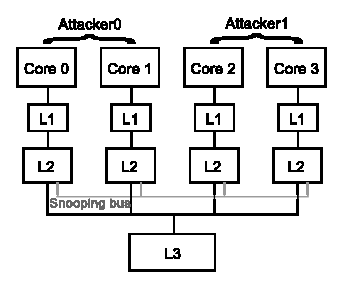
\includegraphics[width=2.3in]{figs/coherent_system.eps}
        \caption{System Configuration}
        \label{fig:coherent_system}
    \end{center}
\end{figure}

Attacker0 has two threads, each running on a different core. Both threads run a $for$ loop of 4000 iterations, and
write to a shared data in each iteration. Before each write is performed, one L2 cache has to forward the data
to the other L2 cache through the snooping bus and invalidates its own copy, according to the cache coherence protocol. 
As a result, there is a lot of coherent traffic between these two threads. Attacker0 runs this $for$ loop repeatedly and
records the time to finish the $for$ loop using c++ timing functions.

Attacker1 owns the secret data ('01101100') and tries to communicate this secret to Attacker0. It checks each bit
in the secret data. If the bit is 0, it executes a $for$ loop which writes to a data in each iteration. This does not produce 
coherent traffic. If the bit is 1, Attacker1 spawns a new thread, which also runs a $for$ loop that writes to the same data, hence producing a lot of coherent traffic. 

\begin{figure}
    \begin{center}
        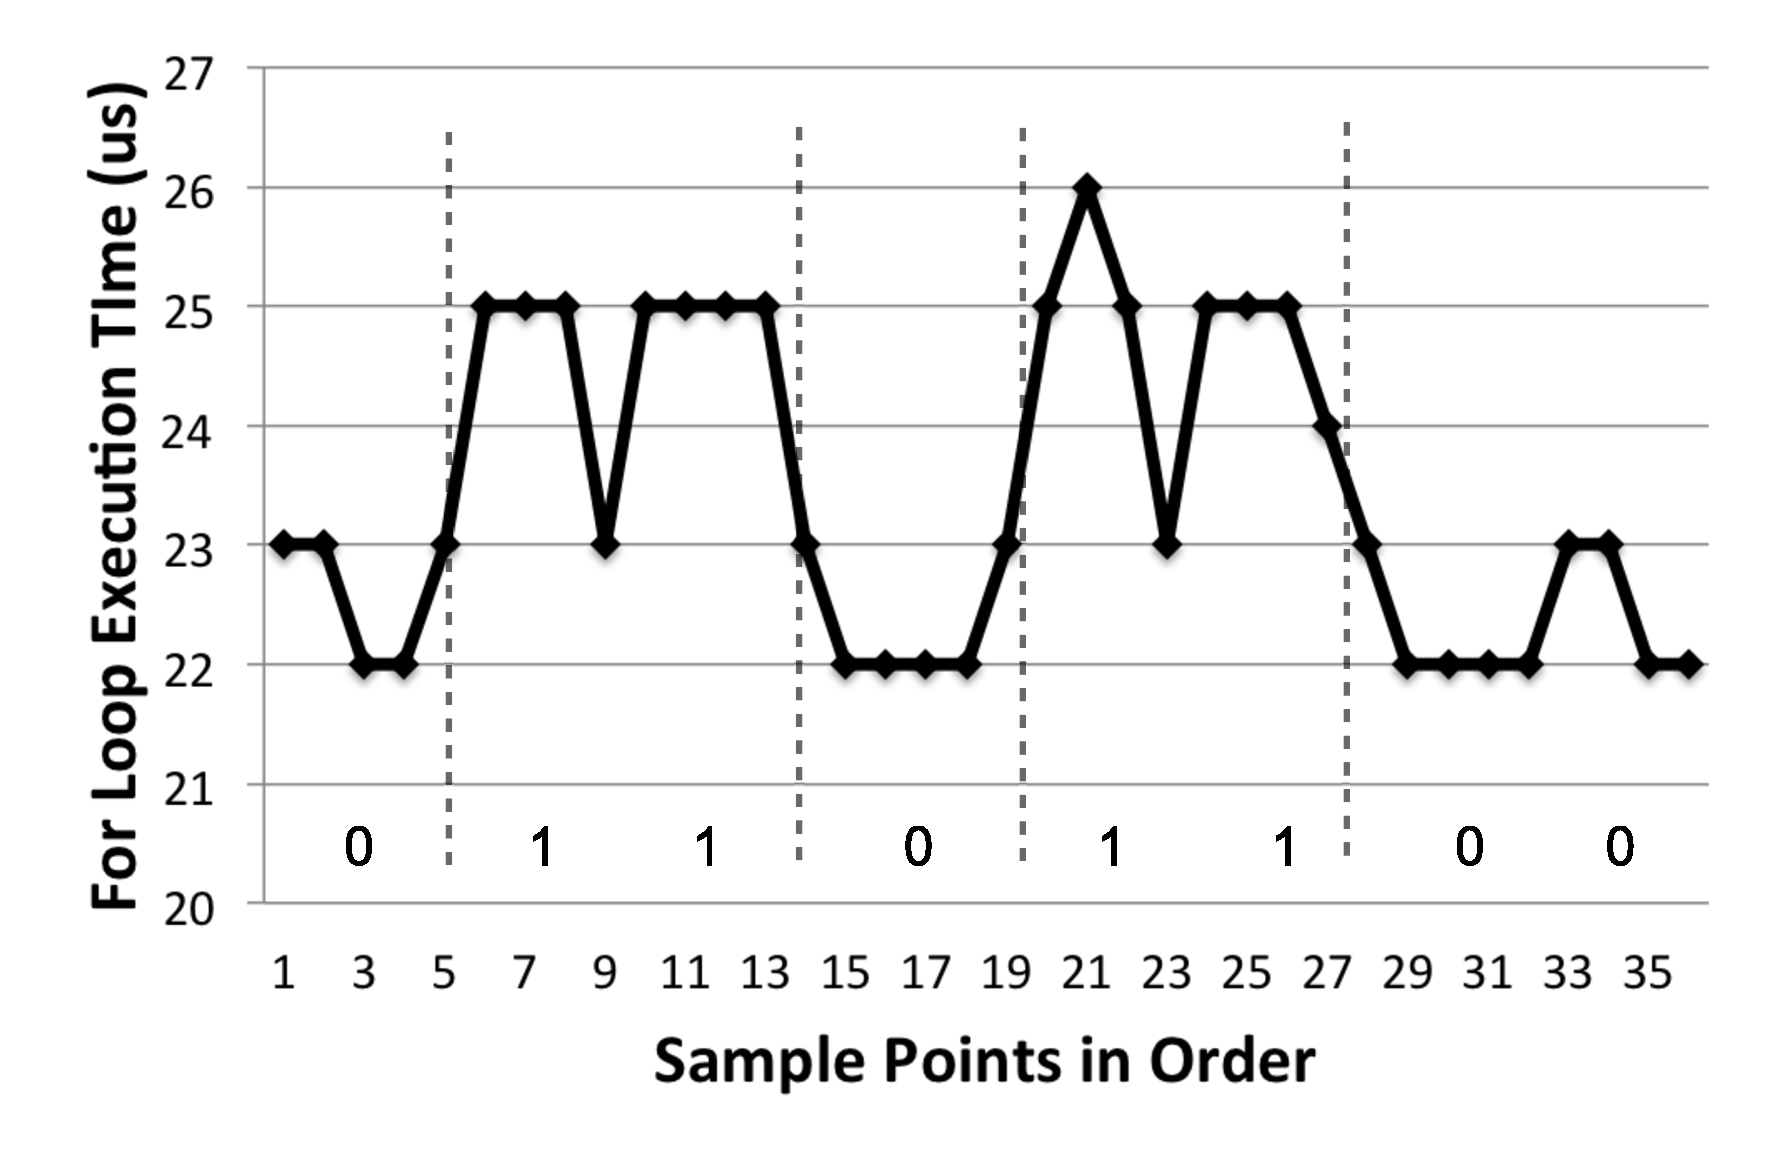
\includegraphics[width=2.79in]{figs/coherence_interference.eps}
        \caption{Attacker0's Timing Observation}
        \label{fig:coherence_interference}
    \end{center}
\end{figure}

Note that in this example, we have all the aforementioned protection schemes implemented except for the snooping bus.
Figure~\ref{fig:coherence_interference} shows the $for$ loop execution time sequence that Attacker0 observes. Each
sample point represents the time it takes to finish a 4000 iteration $for$ loop. Based on the observation, Attacker0
can recover the secret successfully. The timing variation is caused by the interference on the snooping bus. If Attacker1
produces a lot of coherent traffic, Attacker0's coherent traffic gets delayed and thus finishes slower compared to
when Attacker1 does not produce coherent traffic. 

The mechanism to protect against cache coherence timing channels consists of two parts. The first part solves the 
interference on the snooping bus. The snooping bus uses TDM to schedule the snooping requests from different timing
compartments. Each snooping request is attached with a TCID and it can only be sent during its own TC's bus turns.
This protection is the same with what we used for on-chip interconnect. 

The second part deals
with the shared data. Since the shared data is read-only, the cache miss does not necessarily have to be served by
the cache that has the Owned copy. Instead, the cache miss can always be served by the next level of cache or memory.
In our mechanism, when the cache receives a snooping request, it will first check if the TCID of the request matches its
own TCID. If the TCIDs mismatch, then the cache ignores the snooping request even if it has the data, effectively acting
as if the data does not exist. Then the cache miss will be served by the next level of cache. A tricky thing here is
coordinating the operations of multiple level of caches. In some protocols (e.g MOESI), the cache that has the Owned copy
is responsible for responding to the snooping request, so the next level of cache does not respond. In this case, the
cache needs to notify the next level of cache to respond to the snooping request. The notification message should
have a TCID that's the same with the requses so that it does not interfere with its own snooping requests on the snooping 
bus. With our design, the cache that sends a snooping request does not know the data exists on the other cache, while
the timing of the other cache's own operations is not affected.
 
\subsection{Private Per-Core Resources}

The resources that are dedicated to each core such as private caches,
TLBs, and branch predictors, are only used by one timing compartment at a time.
However, multiple timing compartments can use these resources through 
time-sharing. Therefore, there exist state-based timing channels if the state is
kept across context switches. For example, the number of cache blocks that
are evicted by one compartment may affect the number of cache hits for
another compartment in the following time slice.
We eliminate these timing channels by flushing the per-core resource state 
on a context switch that moves to a different timing compartment.
This is handled in software by the timing compartment 
manager (see Section~\ref{sec:integration_tcm}).

\subsection{Other System Resources}

Talk about DMA, I/O, etc. Managed by SW.

%\section{Integration}
Disperate hardware timing channel protection mechanisms are not enough to 
implement a full, timing channel secure system. It requires support from 
software to manage the interaction of software entities with the hardware.  
Further, these hardware mechanisms are often interdependent. The shared cache 
miss path involves the cache, bus, and memory controller, all of which require 
timing channel protection. Haphazardly time multiplexing these resources can 
lead to unnecessarily large performance penalties or even total starvation. The 
integrated system requires carefully coordinating the protected resources. The 
rest of this section elaborates on the timing compartment manager, the software 
entitiy that initializes and manages timing compartments, and then describes 
how timing channel protection mechanisms should be coordinated.

\subsection{The Timing Compartment Manager}
\label{sec:integration_tcm}
The timing compartment manager (TCM) is responsible for initializing and 
managing timing compartments. At system initialization time it informs the 
hardware of the timing compartments present in the system and configures the 
hardware components with the policy. At run time, the TCM tags requests for 
shared hardware resources with the timing compartment ID (TCID) of the TC that 
originated the request. Shared hardware resouces then enforce the policy by 
checking the TCID before handling the request. The hardware allows software 
entities within the same compartment to share resources normally, and timing 
compartments can even be allocated multiple cores.

As shown in Figure \ref{fig:arch}, the timing compartments architecture is 
comprised of a set of $n$ cores which share resources. There is no limitation 
on $m$, the number of timing compartments that can reside in the system at one 
time. However, at most $n$ timing compartments can be active (executing on one 
or more physical cores) at a time. If $m>n$, active timing compartments must 
occasionally be switched with inactive ones. The TCM addresses this by context 
switching TCs according toa context switch schedule.

The TCM is implemented as an extension of the trusted software layer, such as 
the OS or hypervisor. It requires functions to handle the initialization
and context switching. It also requires a small address space of its 
own to store the register contents of inactive TCs and a queue of inactive TCs.
The rest of this section describes the hardware TCID storage elemnts controlled 
by the TCM, and then elaborates on how the TCM initializes the system and 
handles context switching.

\subsubsection{TCIDs}
\begin{figure}
    \begin{center}
        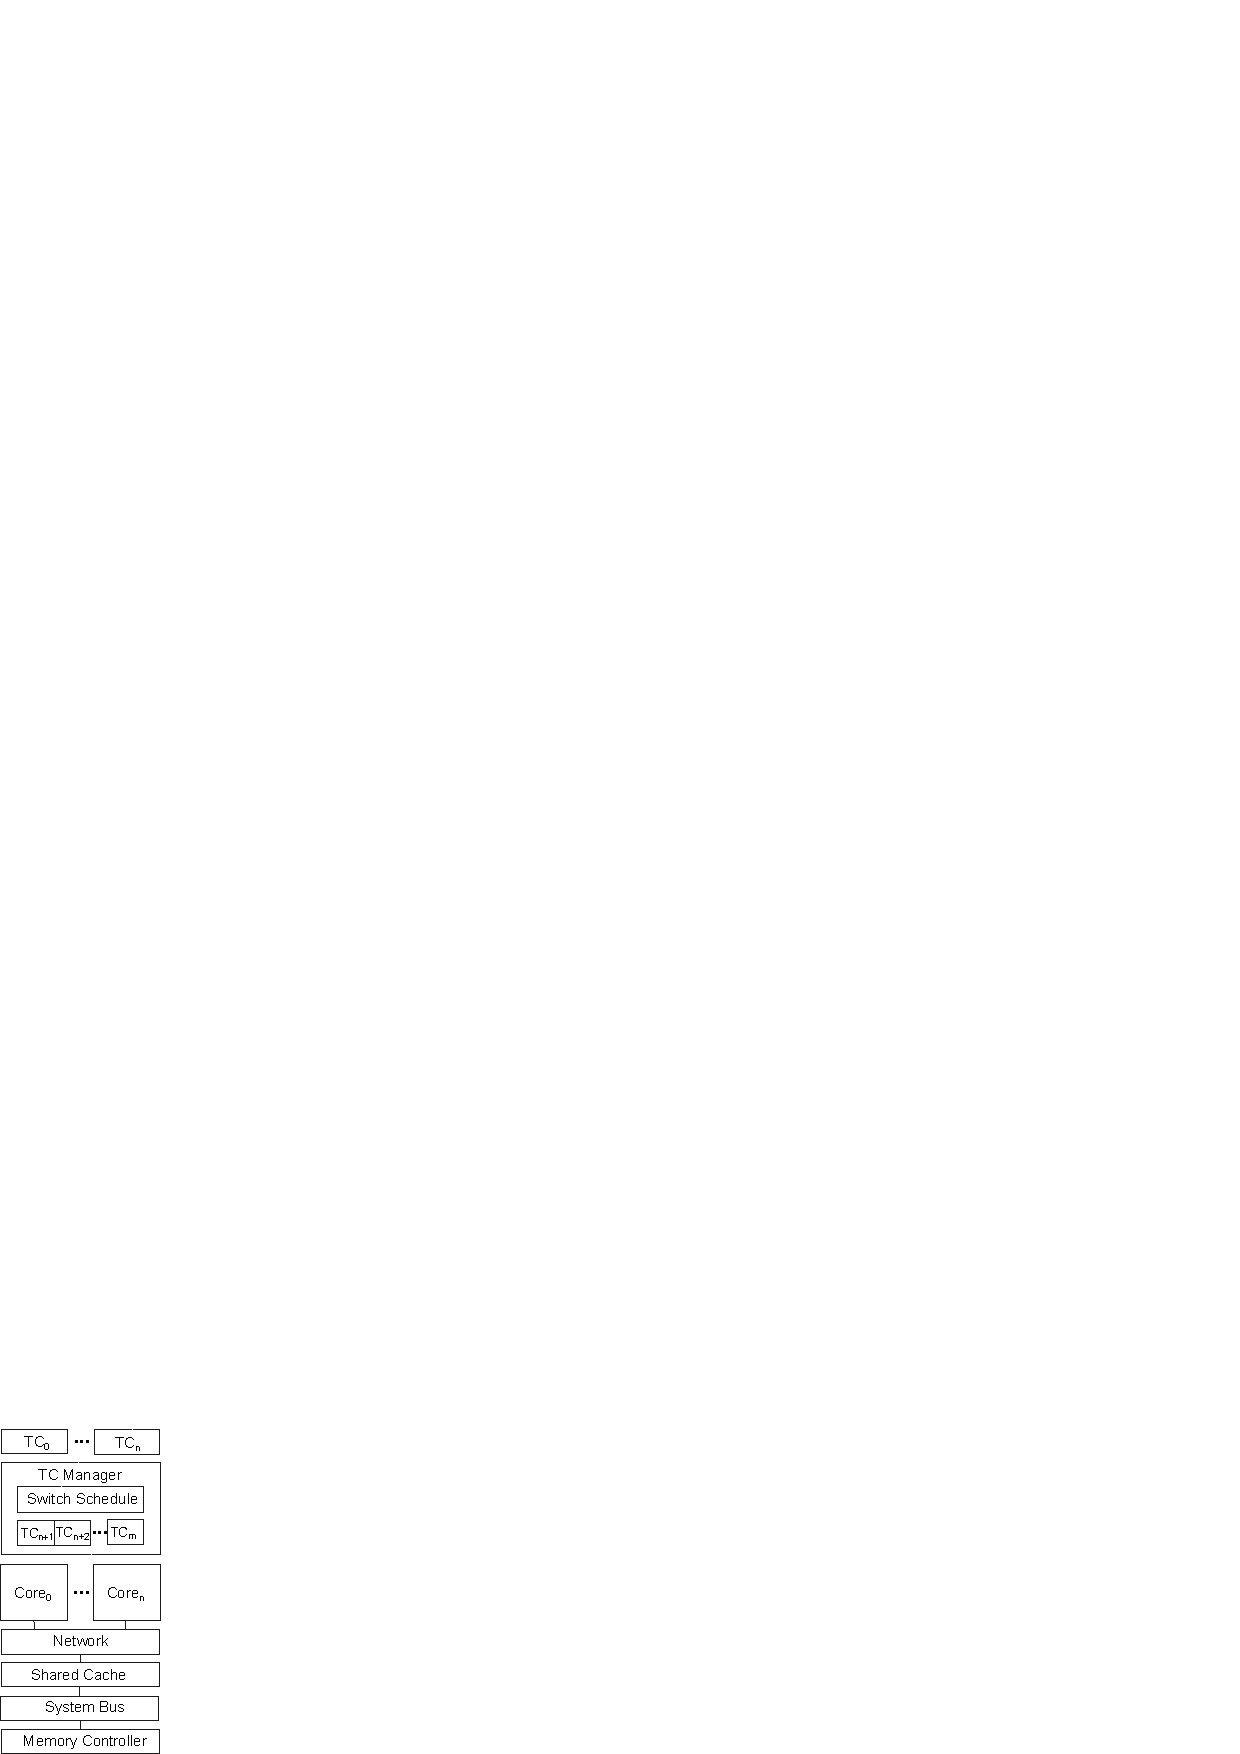
\includegraphics[width=1.08in]{figs/hw_sw_arch.pdf}
        \caption{The Timing Compartments Architecture}
        \label{fig:arch}
    \end{center}
\end{figure}

The hardware protection mechanisms track which timing compartment originated 
each request and handle the requests accordingly. To do so, requests (such as 
network packets or shared cache accesses) are tagged with a timing compartment 
ID (TCID). The set partitioned cache has $n$ registers which store the TCIDs
that own each of the (at most) $n$ partitions. When a request requires a 
replacement, the cache uses the TCID of the request to decide which partitions 
can allow entries to be replaced according to the policy. (Checking is only 
required on replacements since TCIDs have separate address spaces.) Each of the 
separate MSHR banks are tagged with a TCID of the owner, and requests can only 
affect the MSHR banks with the same TCID as the request. Each of the time 
multiplexed resources (the networks, the memory controller, shared cache 
response ports, and memory controller response ports) have $n$ queues. Each of 
these queues has a register to store the TCID which owns that particular queue, 
and time quanta are assigned to each queue. Lastly, each core has a register 
that stores the TCID of the TC currently active on that core. This is used to 
derive the tags that are appended to requests originating from that core. Table 
\ref{table:tcid} summarizes the TCID storage elements in the system.

\begin{table}
\begin{tabular}{l|l}
    \hline
    Component & TCID Storage \\
    \hline
    Core & $n$ cores. TCID register per core. \\
    Shared Cache Port & $n$ queues. TCID register per queue \\
    Shared Cache Parttitions & $n$ partition owner registers. \\
    Shared Cache MSHRs & $n$ MSHR banks. TCID per bank \\
    Network & $n$ queues. TCID register per queue\\
    \hline
\end{tabular}
    \caption{TCID storage for TC Architecture Components}
    \label{table:tcid}
\end{table}

\subsubsection{Initialization \& Handling Context Switches}
The TCM, initializes the system by setting the TCID storage elements listed in 
Table 1 with the IDs of the initially active timing compartments. At most $n$ 
of these can be active initially, so if $m>n$, some will be inactive, and the 
TCM must define a static context switching schedule at initialization time.

The time between context switches cannot depend on the dynamic behaviour of the 
TCs. Otherwise, a timing compartment could observe the time that they are 
context switched in or out to learn information about the timing compartment it 
is switched with. Instead, context switches occur at a fixed time interval, 
$T_{CTX}$. Every $T_{CTX}$ cycles the TCM is invoked to replace the timing 
compartment which has been active the longest with the TC at the head of the 
inactive TC queue. The compartment which has been switched out is moved to the 
back of the inactive TC queue.

To perform the context switch, the CPU pipeline and the memory request queue 
are drained. The general purpose registers of the outgoing TC are stored in 
TCM-space memory and tagged with the TCID. The private cache, shared cache 
partition, TLB, and branch predictor state of the outgoing TC are all flushed.  
Finally, the TCID stores of the outgoing TC are replaced with the TCID of the 
incoming TC. 

The time required to perform a context switch depends on the state and behavior 
of the outgoing TC. The owner of the incoming TC can observe when the incoming 
TC begins executing, so this implies a potential leakage of secrets.  To 
prevent this, context switches are bound to always take the worst case time.  
If a context switch completes early, the incoming TC is stalled until the worst 
case context switch time has been reached.

\subsection{Coordination}

%\section{Cache Coherence Timing Channel}
In a multi-core system, threads are running concurrently on different cores. These threads may share some
data which they read from or write to. The shared data thus can have multiple copies exist in each core's
private cache. In general, a cache coherence protocol is used to ensure each thread gets the most updated
data to work with.

In a snooping-based protocol, the caches on the same level are connected with a snooping bus. When a request
comes into a cache and incurs a cache miss, a snooping request is sent on the snooping bus. All the other
caches observe the snooping request, and one of them may respond to the request by forwarding the data if 
the data exists. The operations to handle snooping requests and responses highly depend on the specific cache 
coherence protocols being used. Commonly used protocols include MSI, MESI and MOESI~\cite{mark_book}.

If different timing compartments share data, there is clearly a timing channel introduced by the cache coherence
protocols. For example, TC0 wants to write to A, and A exists in TC1's cache. In order to perform the write, the
cache coherence protocol will invalidate A in TC1's cache. Later when TC1 wants to read A, it will incur a cache
miss which indicates TC0 has written to A. In our threat model, we assume timing compartments do not share data. 
So the above mentioned timing channel is not a concern. However, our assumption only guarantees the cache state
is not affected by cache coherence protocols. The snooping bus is shared by different timing compartments, thus 
the coherent traffic can still interfere with each other. The interference on the snooping bus introduces timing
channel, as shown in the example below.

\subsection{Covert Channel Attack Example}
In this section, we demonstrate a covert channel attack example on a four-core system. The system configuration 
is shown in Figure~\ref{fig:coherent_system}. Each core has a private L1 and L2 cache, and the four cores share
the L3 cache. The four L2 caches are connected with a snooping bus which uses a MOESI protocol. 
In this example, there are two attackers who
want to communicate a secret data when the direct communication between them is strictly disallowed. Each attacker 
belongs to a different timing compartment. Attacker0 occupies core 0 and core 1 while attacker1 occupies core 2 and
core 3. 

\begin{figure}
    \begin{center}
        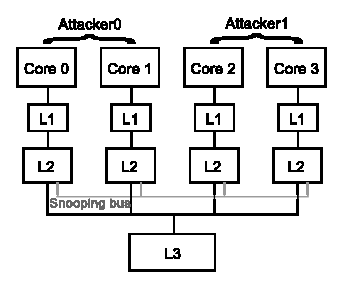
\includegraphics[width=2.3in]{figs/coherent_system.eps}
        \caption{System Configuration}
        \label{fig:coherent_system}
    \end{center}
\end{figure}

Attacker0 has two threads, each running on a different core. Both threads run a $for$ loop of 4000 iterations, and
write to a shared data in each iteration. Before each write is performed, one L2 cache has to forward the data
to the other L2 cache through the snooping bus and invalidates its own copy, according to the cache coherence protocol. 
As a result, there is a lot of coherent traffic between these two threads. Attacker0 runs this $for$ loop repeatedly and
records the time to finish the $for$ loop using c++ timing functions.

Attacker1 owns the secret data ('01101100') and tries to communicate this secret to Attacker0. It checks each bit
in the secret data. If the bit is 0, it executes a $for$ loop which writes to a data in each iteration. This does not produce 
coherent traffic. If the bit is 1, Attacker1 spawns a new thread, which also runs a $for$ loop that writes to the same data, hence producing a lot of coherent traffic. 

\begin{figure}
    \begin{center}
        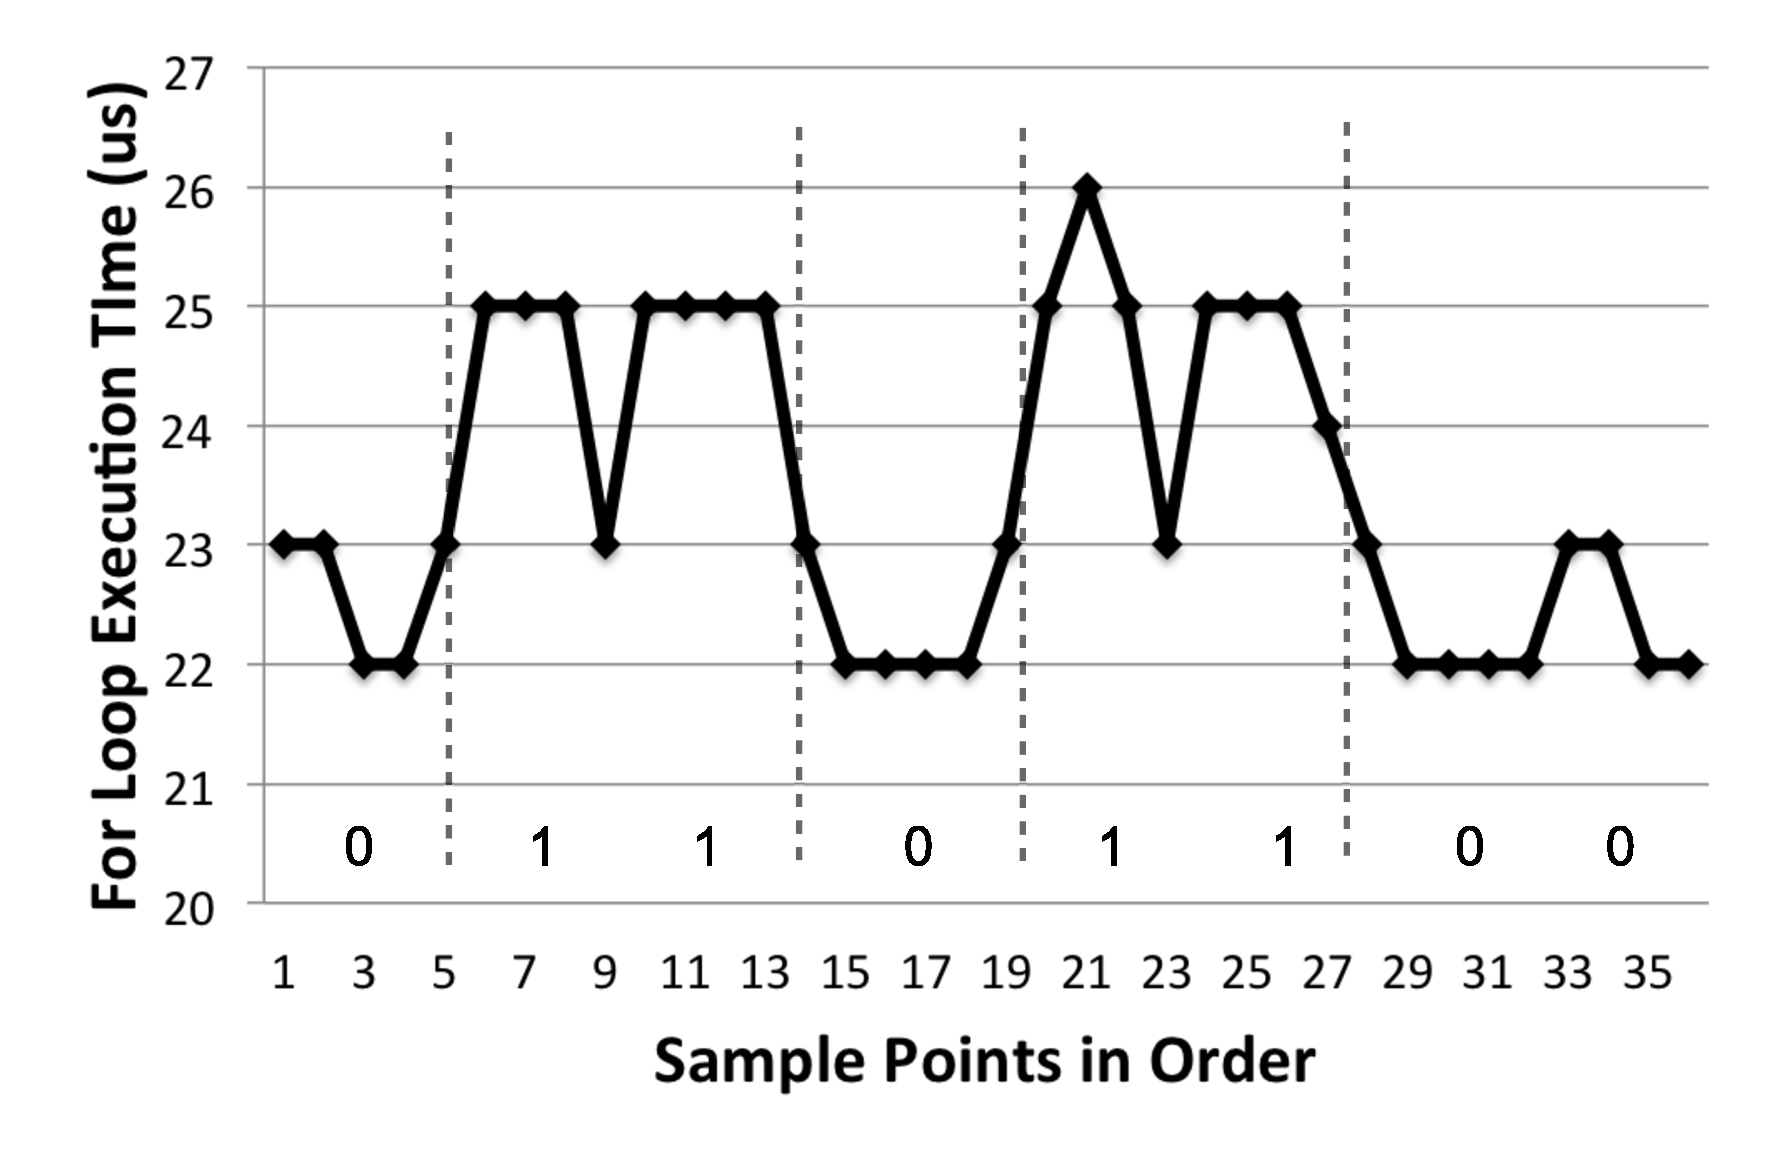
\includegraphics[width=2.79in]{figs/coherence_interference.eps}
        \caption{Attacker0's Timing Observation}
        \label{fig:coherence_interference}
    \end{center}
\end{figure}

Note that in this example, we have all the aforementioned protection schemes implemented except for the snooping bus.
Figure~\ref{fig:coherence_interference} shows the $for$ loop execution time sequence that Attacker0 observes. Each
sample point represents the time it takes to finish a 4000 iteration $for$ loop. Based on the observation, Attacker0
can recover the secret successfully. The timing variation is caused by the interference on the snooping bus. If Attacker1
produces a lot of coherent traffic, Attacker0's coherent traffic gets delayed and thus finishes slower compared to
when Attacker1 does not produce coherent traffic. 

\subsection{Protection Scheme}
The protection scheme is similar to the normal bus protection. We attached the TCID to the snooping requests and responses.
The snooping bus scheduling is changed to round-robin scheduling. With this protection, the coherent traffic from different
timing compartments do not interfere with each other through the snooping bus. This protection prevents the covert channel
attack mentioned above.

%%%%%%%%%%%%%%%%%%%%%%%%%%%%%%%%%%%%%%%%%%%%%%%%%%%%%%%%%%%%%%%%%%%%%%%%%%%%%%%
%% Outline
%%%%%%%%%%%%%%%%%%%%%%%%%%%%%%%%%%%%%%%%%%%%%%%%%%%%%%%%%%%%%%%%%%%%%%%%%%%%%%%
% 
% Explain problem without timing details. Use figure that has turn lengths with 
% no offsets. Show a packet traversing through path with latencies outlined and 
% the packet getting delayed. Explain figure.
% 
% Though the l3 hit path is simple, whole l2 miss path is a nontrivial problem 
% - many tradeoffs, used linear optimization. Wrote simulator to explore this.  
%   Ultimately found a general scheme
% that an optimizer couldn't beat for the l3 miss path. Finding agood balance 
% between
% the hit and miss paths required an optimizer and we did not find a general 
% scheme
% 
% \subsection{L2 Miss Timing Sequence}
% Introduce l3 hit timing sequence with figure. Explain figure.
% 
% Show l3 miss timing sequence. Use figure.
% 
% \subsection{Latency Simulator \& Optimal Coordination}
% 
% Explain goal of coordinating (EV of L2 miss latency). Usually achieved by 
% aligning turns of adjacent devices. Use turn lengths (duration a TC is 
% scheduled to use a device - depends time to send message, affects 
% ``randomness'' of schedule) and offsets (difference in start times that
% improves how the schedule relates to the schedule of other devices).
% 
% Show how to optimize l3 hits. Use figure.
% 
% Explain tradeoffs. Use figure?? It is not simple to solve.
% 
% Wrote our own l2 miss (l2 to l2) timing simulator. Explain what it simulates.  
% (Assumes uniform random arrival, calculate latency for every possible arrival 
% in a schedule, gets EV of latency).
% 
% Exhaustive search of L3 hit path. Confirms that an intuitive design is best.
% 
% Cannot exhaustively search L3 miss path latencies. Instead use linear 
% optimizatin. Search space has many relative minima (change offset slightly, 
% suddenly schedule is much better) - cannot use hill climbing. Use simulated 
% annealing. Explain our simulated annealing implementation. Optimize for l3 
% miss alone and l2 miss latency assuming hit rate of 90\%.
% 
% Tried a scheme we suspected would have a good L3 miss latency. Optimal result 
% was different. Adjusted optimizer result to something that made more 
% intuitive sense and iterated. Reran optimizer on result of iterative 
% approach, and the optimizer could not find a better scheme in 20,000 steps.
% 
% Explain optimal scheme. Use figure.
% 
% For l2 miss latency, no intuitive general approach could be found. Balance 
% between hit/miss paths is difficult.


%%%%%%%%%%%%%%%%%%%%%%%%%%%%%%%%%%%%%%%%%%%%%%%%%%%%%%%%%%%%%%%%%%%%%%%%%%%%%%%
%% Old Figures
%%%%%%%%%%%%%%%%%%%%%%%%%%%%%%%%%%%%%%%%%%%%%%%%%%%%%%%%%%%%%%%%%%%%%%%%%%%%%%%
% \begin{figure}
%     \begin{center}
%         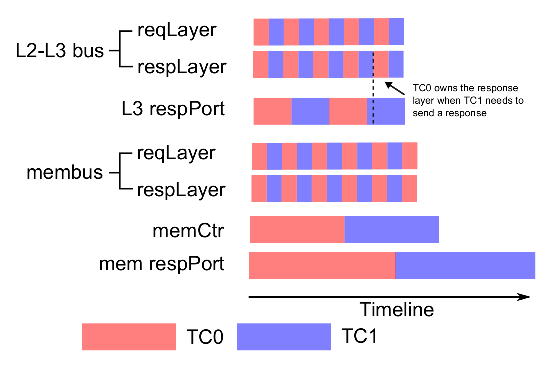
\includegraphics[width=3.46in]{figs/baseline_schedule.eps}
%         \caption{Cache hit timing sequence.}
%         \label{fig:naive_scheme}
%     \end{center}
% \end{figure}
% 
% 
% \begin{figure}
%     \begin{center}
%         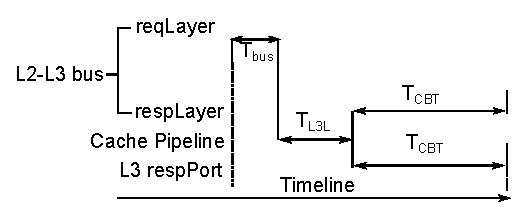
\includegraphics[width=2.4675in]{figs/hit_timing.eps}
%         \caption{L3 cache hit timing sequence.}
%         \label{fig:hit_timing}
%     \end{center}
% \end{figure}
% 
% \begin{figure}
%     \begin{center}
%         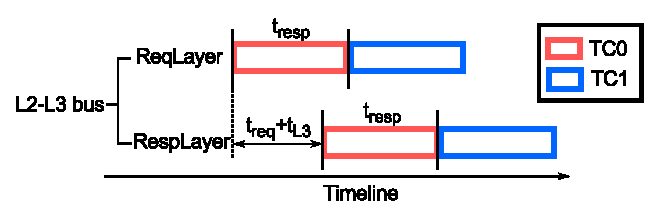
\includegraphics[width=3.2624in]{figs/hit_schedule.eps}
%         \caption{Cache hit timing path schedule.}
%         \label{fig:hit_schedule}
%     \end{center}
% \end{figure}
% 
% \begin{figure}
%     \begin{center}
%         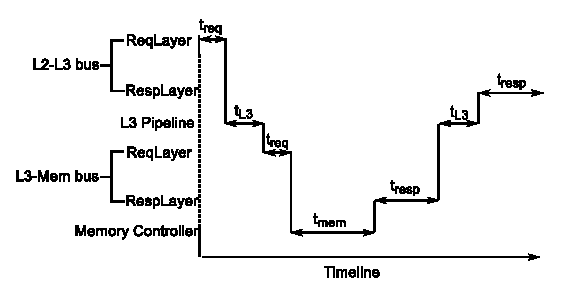
\includegraphics[width=2.9475in]{figs/miss_timing.eps}
%         \caption{The L3-memory timing sequence.}
%         \label{fig:miss_timing}
%     \end{center}
% \end{figure}
% 
% \begin{figure}
%     \begin{center}
%         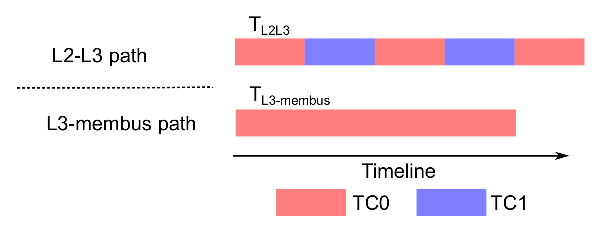
\includegraphics[width=2.9475in]{figs/coordination.eps}
%         \caption{A coordinated cache miss path schedule.}
%         \label{fig:coordination}
%     \end{center}
% \end{figure}

\section{Time Slice Coordination}
The Timing Compartments architecture relies heavily on time multiplexing to 
protect shared resources including the L2-L3 bus, the L3-memory bus, and the 
memory controller. These resources frequently interact since each is involved 
in handling L2 misses. If the time multiplexing schedules for each of these 
resources are not designed to account for this interaction, it could lead to 
exorbitant latencies and wasted bandwidth.

\begin{figure}
    \begin{center}
        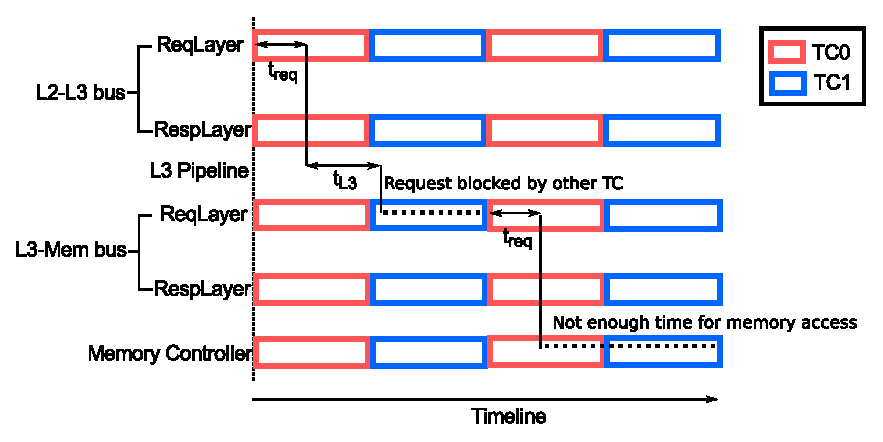
\includegraphics[width=3.46in,height=2in]{figs/problem.eps}
        \caption{A poorly performing time multiplexing schedule.}
        \label{fig:problem}
    \end{center}
\end{figure}

Figure \ref{fig:problem}, illustrates the problem. It shows when each of two 
timing compartments are scheduled to use the time multiplexed resources along 
the L2 miss path. Red blocks indicate that TC0 is scheduled to use the device, 
and blue blocks indicate that TC1 is scheduled. We refer to the block of time 
that a timing compartment is scheduled to use a device as the \emph{turn} and 
we refer to the duration of a turn as the \emph{turn length}. In this schedule, 
timing compartments are allotted the same turn length for each time multiplexed 
resource, and the schedule for each device starts at the same time.

%%%%%%%%%%%%%%%%%%%%%%%%%%%%%%%%%%%%%%%%%%%%%%%%%%%%%%%%%%%%%%%%%%%%%%%%%%%%%%%
%% This section is easier to write if we introduce bus layers in the uarch 
%% channel section (section 3)
%%%%%%%%%%%%%%%%%%%%%%%%%%%%%%%%%%%%%%%%%%%%%%%%%%%%%%%%%%%%%%%%%%%%%%%%%%%%%%%
An L3 miss from TC0 is shown proceeding with these time multiplexing schedules.
The miss begins at the L2 request layer where the request is sent to the L3.  
When the L3 access is complete, the request must proceed through the L3-memory 
bus request layer, but at this time TC1 is scheduled to use the L3-memory 
request layer, so it must wait for TC1's turn to finish before the request can 
proceed to the memory controller. There are similar issues as the packet 
traverses the rest of the path.

Clearly, this schedule is inefficient. When designing a schedule for these 
resources both the L3 hit and L3 miss paths should be considered. In this 
section we describe the timing for both paths. We then show that devising a 
schedule that optimizes just the hit path is straightforward, but scheduling 
the miss path and balancing both is challenging.

\subsection{L2 Miss Timing Paths}
Naturally, to efficiently time multiplex the resources involved in an L2 miss, 
understanding the timing of L2 misses is key. L2 misses take two different 
paths and have different timings depending on whether the L2 miss is an L3 hit 
or miss. Figure \ref{fig:hit_timing} shows the timing for an L3 hit. The arrows 
indicate the time that the resource in the corresponding column is used.

The L2 miss begins by transferring a request over the L2-L3 bus request layer 
in $t_{req}$ cycles. Typically, $t_{req}$ depends on how the bus protocol 
requires requests to be sent. The request then arrives at the L3 cache, where 
it takes $t_{L3}$ cycles (i.e. the L3 cache latency). We assume the cache is 
fully pipelined, so even if a request arrives one cycle after another, both can 
use the cache simultaneously, and the access always completes in $t_{L3}$ 
cycles. Finally, the data is transferred from the L3 response port back to the 
L2 over the L2-L3 bus response layer in $t_{resp}$ cycles. Often, $t_{resp}$ 
will be greater than $t_{req}$. It depends on the bus bandwidth and the size of 
a cache block.

\begin{figure}
    \begin{center}
        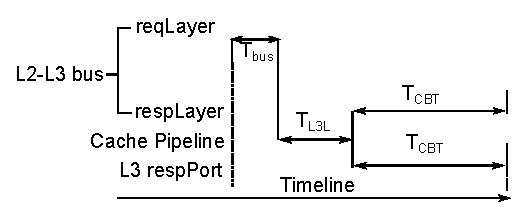
\includegraphics[width=2.4675in]{figs/hit_timing.eps}
        \caption{L3 cache hit timing sequence.}
        \label{fig:hit_timing}
    \end{center}
\end{figure}

Figure \ref{fig:miss_timing} shows the timing for an L3 miss. The request 
begins by transferring over the L2-L3 bus request layer, and similarly takes 
$t_{L3}$ cycles to identify that it is a miss. Afterwards, it sends another 
request to the memory controller over the L3-memory bus request layer in 
$t_{req}$ cycles. Memory requests take variable time to complete, after which 
the data is returned to the L3 in $t_{resp}$ cycles, written to the L3 in 
$t_{L3}$ cycles and finally returned to the L2 after another $t_{resp}$ cycles.

\begin{figure}
    \begin{center}
        \includegraphics[width=2.9475in,height=1in]{figs/miss_timing_v2.eps}
        \caption{L3 cache miss timing sequence}
        \label{fig:miss_timing}
    \end{center}
\end{figure}

\subsection{Devising a Schedule}
A good time multiplexing schedule should minimize the L2 miss latency for most 
cases. We can achieve this by controlling the turn lengths and offsets for each 
time multiplexed device. Here, an \emph{offset} refers to a shift in the start 
of the schedule for a single device. Offsets are used to make a resource 
available precisely when the data is available from the preceding resource.

%% A schedule is determined by the set of turn lengths and offsets for each 
%% resource. Turns are allocated for each timing compartment in a repeated 
%% sequence (e.g. 1,2,3,4,1,2,4, for four timing compartments). Therefore, a 
%% schedule for the entire path repeats after the least common multiple of each 
%% turn length in the path multiplied by the number of timing compartments. The 
%% latency for a request can be 

For a particular resource, suitable turn lengths depend on the latency of that 
resource, and suitable offsets depend on the latency of the preceding resource.
This reasoning can be applied in a straightforward way to derive the schedule 
that optimizes the L3 hit path shown in Figure~\ref{fig:hit_schedule}.

The turn length for the L2-L3 request layer must be greater than $t_{req}$. The 
data is available to the L2-L3 response layer after $t_{req}+t_{L3}$ cycles, so 
this is used as the offset for the response layer. The turn length for the 
response layer is $t_{resp}$. Since typically $t_{req}<t_{res}$ we could use a 
shorter turn length for the request layer. However, any requests from one TC 
would be queued until the turn for the same TC on the response layer starts, so 
this provides no benefit. In fact, reducing the turn length causes requests 
that arrive later in the schedule to incur extra delays.

\begin{figure}
    \begin{center}
        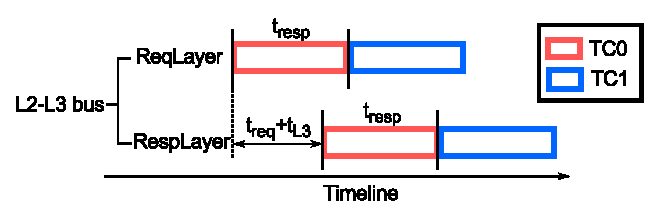
\includegraphics[width=3.2624in]{figs/hit_schedule.eps}
        \caption{Cache hit timing path schedule.}
        \label{fig:hit_schedule}
    \end{center}
\end{figure}

Scheduling the L3 miss path is more complicated. The miss path involves two 
more bus layers and the memory controller. The memory accesses take much longer 
than bus transfers and the turn lengths for both can have a large least common 
multiple. As we will show, this can make L2 miss latencies unpredictable if not 
handled well. Further, the memory controller requires a dead time to drain 
in-flight requests and prevent interference. New requests cannot begin during 
the dead time, but old ones can continue. Memory requests must also finish in a 
single turn complicating the schedule even further.

To find the schedule that optimizes the miss path, we used a mix of intuitive
reasoning and integer linear programming optimization techniques, as discussed 
in Section \ref{sec:eval_coord}.
The turn lengths for both L3-memory bus layers and the memory controller are 
$t_{mem}$, the minimum memory turn length. Although these bus turns could have 
been smaller, this would provide no benefit since they transfer responses to 
and from the memory controller exclusively. The L2-L3 bus layer turn lengths 
were the smallest factor of $t_{mem}$ greater than $t_{req}$. The scaling is 
beneficial since the least common multiple of turn lengths affects the
repeatability of the schedule. The L2-L3 bus turns are increased rather than 
the memory controller since this schedule only optimizes the L3 miss path, not 
the entire L2 miss path. Each device schedule is offset so that it starts when 
the data is available. Table \ref{tab:config} summarizes both the turn lengths 
and offsets in this schedule. Here $t_{read}$ is the worst case memory read 
time.

Scheduling the full L2 miss path is even more difficult. Typically getting a 
schedule that repeats in a short period requires increasing either the L3 hit
or miss path. We examined this scheduling problem with linear optimization 
techniques, and although we could not construct much meaning from the optimal 
schedule, we will show in Section \ref{sec:eval_coord} that the gap between
the best and worst schedules is significant. This suggests that although time 
multiplexing the L2 miss path is a difficult problem, it can greatly impact 
performance.

\section{Evaluation}

We evaluated the timing compartments architecture using the gem5 architectural 
simulator~\cite{gem5} integrated with the DRAMSim2~\cite{DRAMSim2} 
memory simulator. Our experiments use multiprogram workloads 
comprised of SPEC2006 benchmarks compiled for the ARM ISA. 

Table~\ref{tab:config} shows our system configuration.
The cores use the gem5 ``O3`` out-of-order core model which runs at 2GHz. 
Each core has private 32KB L1 instruction and data caches, and private 256KB L2 
cache. The cores share a 4MB L3 cache. We derived cache configuration 
parameters from the Intel Xeon E3-1220L, which is a two core architecture used 
by Amazon EC2. In DRAMSim2, we simulate a 667MHz 2GB DDR3 memory. The 
interconnects in the simulator runs at 1GHz. Unless specified otherwise, each experiment is 
fastforwarded for 1 billion instructions, and run for 100 million 
instructions. We will first describe our security evaluation and then show
the performance evaluation.

\begin{table}
    \caption{Simulator configuration parameters.}
    \centering
    \begin{tabular}{|l|l|l|r|}
        \hline
        \multicolumn{3}{|l|}{gem5 core model} & ``O3''        \\\hline
        \multicolumn{3}{|l|}{CPU Clock}    & 2GHz             \\\hline
        \hline
        \multicolumn{2}{|l|}{Memory}             & 2GB    & 667MHz  \\\hline
        \hline
        \multicolumn{3}{|l|}{Network Clock}      & 1GHz \\\hline
        \hline
        L1d / L1i  & 32kB   & 2-way  & 2 cycles\\\hline
        L2         & 256kB  & 8-way  & 7 cycles \\\hline
        L3         & 4MB    & 16-way & 17 cycles  \\\hline
    \end{tabular}
    \label{tab:config}
\end{table}

\subsection{Security Evaluation}

To experimentally evaluate the security of the timing channel protection in our 
architecture, we use a two-core system with two timing compartments, TC0 and
TC1, running concurrently. The protection policy is configured to disallow any 
timing channels between the two compartments. If the number of cycles required 
to execute a certain number of instructions for a particular benchmark running on 
TC0 depends on which benchmark is running on TC1, it indicates timing 
interference exists that can be exploited to leak information about TC0. A 
secure system should guarantee the benchmark running in TC0 always uses the 
same number of cycles to finish regardless of which benchmark TC1 is running. 

Using the rule above, we evaluated the security of our architecture by running 
a fixed benchmark on TC0 while varying the benchmark on TC1. Then we compared 
the total execution time for the fixed benchmark in different runs. We 
evaluated our architecture as well as the baseline insecure architecture which 
does not implement any protection. As expected, the results for the baseline 
show the execution time of a particular benchmark on Core 0 changes significantly 
depending on the benchmark on Core 1, indicating timing channels exist between
the two cores. On the other hand, when running each pair of benchmarks with 
timing channel protection we observed no execution time difference by changing 
which program runs concurrently with TC0.

\subsection{Time Slice Coordination}
\label{sec:eval_coord}
We analyzed the L2 miss path TDM scheduling problem using our own simulator.
Given the turn lengths and offsets of each device, the latency of a request can be 
determined based on the cycle in which a request arrives in the schedule.
Since a schedule repeats after the least common multiple of each 
turn length in the schedule multiplied by the number of timing compartments, 
each possible latency for a schedule can be enumerated. The simulator finds
each possible latency in a schedule, and calculates the 
expected value of this latency assuming the arrival time at the L2-L3 bus is 
uniform random.

Using this simulator, we exhaustively searched for the optimal L3 hit path 
schedule with the parameters summarized in table ~\ref{tab:coord_param}. The 
search space includes turn lengths from 1-25 cycles and all possible offsets 
for each turn length. We confirmed that the intuitive schedule described in 
Section \ref{sec:coordination} achieves the highest expected value of the 
latencies for L2 misses that hit in the L3.
Fixing the turn lengths to the optimal ones and adjusting only the offsets,
the worst case latency is 19.6\% worse than the optimal schedule, showing
that coordinating the hit path is important.

\begin{table}
    \caption{Time slice coordination simulator paramaters}
    \centering
    \begin{tabular}{|r|r|}
        \hline
        $t_{req}$  &   1 cycle \\\hline
        $t_{resp}$ & 9 cycles \\\hline
        $t_{L3}$   &   9 cycles \\\hline
        $t_{read}$ & 36 cycles \\\hline
    \end{tabular}
    \label{tab:l2_miss_schedules}
\end{table}

The search space for schedules involving every resource in the L2 miss path
is far too large to search exhaustively.
Instead we used integer linear programming optimization 
techniques. Changing a turn length or offset slightly can drastically affect 
the performance, so the search space has many relative minima. We used 
our own simulated annealing optimizer to avoid getting stuck at relative minima 
and increase our chances of finding a global minimum.

We used the optimizer to 
study the latency of L2 misses that miss in the L3.
After initializing the optimizer with the L3 miss schedule summarized in 
Figure~\ref{fig:miss_schedules}, the optimizer did not find a 
better schedule after 20,000 iterations. Fixing the turn lengths to be the same 
as the best schedule found and sweeping only the space of offsets,
the worst-case schedule performed 2.38X
worse than the optimal schedule.

We used the same optimizer to study the latency of L2 misses in general 
assuming a 90\% L3 cache hit rate.
Optimizing for the L2 miss rate overall is a harder problem since it requires a balance 
bewtween the best L3 miss case and L3 hit case parameters. The 
schedule produced by the optimizer was not one that made any intuitive sense. 
However, the optimal schedule was 8.67X better than the worst schedule that 
used the same turn lengths as the best schedule (and changed only the offsets).

The results for schedule selection study are summarized in Table 
\ref{tab:coord_results}. Overall, scheduling 
interdependent time multiplexed devices is a challenging problem, but the gap 
between the worst and optimal cases show that it is important.

\begin{table}
    \caption{Scheduling Selection Study Results.}
    \centering
    \begin{tabular}{|l|l|l|l|}
        \hline
        \multicolumn{1}{|l|}{Optimized Quantity} & Search & Min & Max \\\hline
        \multicolumn{1}{|l|}{L3 Hit Latency} & Exhaustive & 25.5 & 30.5 \\\hline
        \multicolumn{1}{|l|}{L3 Miss Latency} & Simulated Annealing& 139.5 & 334.5 \\\hline
        \multicolumn{1}{|l|}{L2 Miss Latency} & Simulated Annealing& 38.6 & 344.5 \\\hline
    \end{tabular}
    \label{tab:coord_results}
\end{table}

\subsection{Performance Evaluation}

The timing compartment architecture extends the insecure baseline with
static partitioning and time multiplexing to secure the shared hardware 
resources. These changes lead to underutilization, and thus, a performance
overhead. To evaluate the performance overhead, we ran pairs of
SPEC2006 benchmarks, and measured the execution time of the benchmark
in TC0. Since the timing channel protection mechanisms primarily affect the memory 
hierarchy, the memory intensity of the benchmarks is related to the performance 
overhead.
The memory intensity of each benchmark, in memory requests per thousand 
instructions, during the program segment used for our experiments is shown in
Figure~\ref{fig:memstudy}. Of the SPEC2006 benchmarks, mcf has the most memory 
requests, while astar has none after fast-forwarding for 1B instructions.

For the baseline architecture, we calculate the average execution time of the 
benchmark on Core 0 by averaging among runs with different benchmarks on Core 1. 
The execution time of the benchmark in Core 0 is impacted by the benchmark in 
Core 1. In the timing compartments architecture, the execution time of TC0 (on 
Core 0) is independent of workloads running in other timing compartments.

\begin{figure}
    \begin{center}
        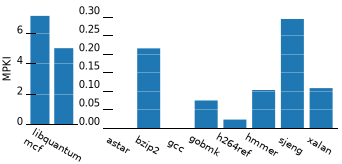
\includegraphics[width=3.4in]{figs/mpki_merged.pdf}
        \caption{Memory intensity of SPEC2006 benchmarks.}
        \label{fig:memstudy}
    \end{center}
\end{figure}

Figure~\ref{fig:performance} shows the performance overhead of full system 
protection as well as the overhead incurred by the changes to the memory 
controller (mc), the cache (waypart), the L3 to memory bus (membus), and the L2 
to L3 bus (L2L3) individually compared to the insecure baseline. The
overheads for libquantum and mcf, which are particularly memory intensive, are 
highest at 69\% and 18\% respectively. However, the arithmetic mean of the 
total overhead is quite low at roughly 9\%. Memory controller protection incurs 
by far the most overhead suggesting the impact on memory bandwidth is more 
significant than bus or cache underutilization. Overall, the results show that 
the timing compartments are viable for applications that require high assurance 
for software isolation.

\begin{figure}
    \begin{center}
        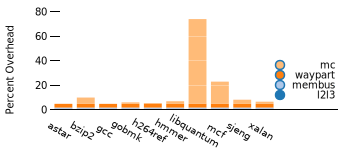
\includegraphics[width=3.4in]{figs/breakdown.pdf}
        \caption{Performance overhead for 2 TCs.}
        \label{fig:performance}
    \end{center}
\end{figure}

The performance overhead is likely to increase as the number of timing 
compartment scales up. To study the impact of the number of timing 
compartments, we evaluated the performance overhead with three and four timing 
compartments on a 4-core  processor, each occupying one core and private L1 and 
L2 caches. They share a 4MB L3 cache. We do not evaluate all permutations of 4 
benchmarks. Instead, we only evaluate the subset of these permutations where 
TC1, TC2, and TC3 are executing the same benchmark. As before, each of these 
workloads with the same program in TC0 is averaged.

The performance overhead as the number of timing compartments increases is 
shown in Figure~\ref{fig:scalability}. The arithmetic mean of the overheads for 
each benchmark for 2, 3 and 4 timing compartments are 9\%, 17\%, and 24\% 
respectively. For libquantum which is particularly memory intensive, the 
overheads are 76\%, 140\%, and 184\% for 2, 3, and 4 timing compartments. The 
results suggest that the overhead of timing timing channel protection is rather 
insensitive to the number of timing compartments for compute-bound 
applications. For memory-intensive applications, the overhead can increase 
noticeably. However, the results still suggest that timing compartments can 
allow distrusting software entities to share hardware and provide better 
overall performance than running them on separate dedicated machines.

\begin{figure}
    \begin{center}
        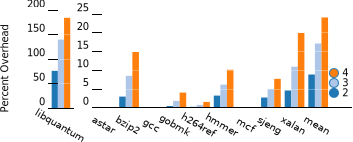
\includegraphics[width=3.4in]{figs/scalability_split.pdf}
        \caption{Performance overhead for 4 TCs.}
        \label{fig:scalability}
    \end{center}
\end{figure}

While future multi-core systems are likely to have a large number of processing 
cores, we note that many security applications will not require many timing 
compartments to be used concurrently. For example, the BYOD application only 
requires two TCs no matter how many cores exist in the system. Similarly, in 
a high-assurance cloud computing environment, the cloud provider can limit the
number of high-assurance virtual machines that can be located on each physical
system while increasing the system utilization by co-locating non-secure
virtual machines with high-assurance ones.

\subsection{Cache Coherence Performance Overhead}
Adding the timing channel protection for snooping bus can introduce some performance overhead. We evaluate some 
splash2~\cite{splash2} benchmarks in gem5. The system we model is the one shown in Figure~\ref{fig:coherent_system}.
We use the same splash2 benchmarks for Attacker0 and Attacker1, each consists of two threads. We terminate the simulation
when thread on core 0 reaches 100M instructions. 
Our baseline is a system where every other timing channel protection scheme we proposed is implemented except for the snooping bus.
We then compare it with the system where the snooping bus is also protected. This comparison enables us to quantify the exact overhead introduced by adding cache coherence protection. 

The results are shown in Figure~\ref{fig:splash2}. As can be seen, the overhead of adding cache coherence protection is
quite low, with the highest overhead less than 1.5\%. In some cases the protection scheme even outperform the baseline, 
mainly because the round-robin scheduling may have avoided some snooping bus contention in the baseline scheduling. 
The main reason for the low overhead is that the coherent traffic is quite rare in programs, hence the round-robin
snooping bus will not cause much overhead to the overall program execution time.

\begin{figure}
    \begin{center}
        \includegraphics[width=2.79in]{figs/splash2.pdf}
        \caption{Performance Overhead of Cache Coherence Protection}
        \label{fig:splash2}
    \end{center}
\end{figure}

\section{Related Work}

Previous studies identified 
a number of microarchitectural timing channels 
caches~\cite{percival,bernstein,caseofaes,remoteaes,analyticalcache,collision,
deconstructing,cachegames}, branch predictors 
\cite{branchpred,predictingbranch}, processor
pipelines \cite{pipelines}, networks on chip~\cite{yaonocs,surfnoc}, and memory
controllers~\cite{ushpca14,fletcher-hpca14}. 
Also, people have proposed solutions for timing channels in
individual components such as caches~\cite{newcache,deconstructing}, memory
controllers~\cite{ushpca14,fletcher-hpca14}, and on-chip network
~\cite{yaonocs,surfnoc}.
However, the previous work has
so far focused on individual component. This work represents the first attempt
at designing a full microprocessor with complete internal timing channel protection.
Our integration efforts also exposed new sources of timing channels in module
interfaces such as MSHRs and cache/memory response ports.

%However, this paper presents the first microarchitecture to address all 
%internal microarchitectural timing channels. 

Ascend~\cite{ascend} proposes a
microarchitecture that aims to eliminate external timing channels so that
even untrusted software can execute without leaking any confidential
data. This presents a powerful option if physical attacks need to be
considered. However, Ascend does not allow a processor to be shared by
multiple software components at the same time, and does not address 
any internal timing channels.
Execution leases~\cite{execution_leases} 
provide another external timing channel solution at the hardware level by 
enforcing strict upper bounds on the execution times of program subsections. 

Timing channels are a form of information flow, and there is a large body
of work on information flow control. For example, language-level approaches
track information flow that is visible at the program level to either 
eliminate~\cite{quantleaks} or 
reduce~\cite{mitigation1,mitigation2,mitigation3} timing channels. 
However, language-level approaches cannot fully control microarchitecture-level
timing channels because traditional instruction set architecture hides
timing inside a processor.
At the 
systems level, information flow control has been used to control
explicit communication channels~\cite{flume-sosp07,histar-sosp06,laminar-pldi09}. 
These software approaches can control explicit information flows or external
timing channels that the timing compartments do not handle.
The timing compartments complement these software approach by
controlling microarchitectural timing channels.

There have been recent efforts on verifying information flow properties
of hardware including certain timing channels. For example, GLIFT
\cite{glift-asplos09} dynamically tracks all information flows, including timing channels,
at the logic gate level. 
The idea in GLIFT has been extended to develop verifying
information flow properties using gate-level simulations
\cite{glift-dac10,glift-dac11,glift-isca11} and a 
hardware description language
~\cite{caisson-plas10,caisson-pldi11,sapper-plas13}.
However, these approaches so far have only been applied to simple
processors and a very strict isolation mechanism. 
This paper studies timing channel protection on complex multi-core processors.


\section{Conclusion}
This paper presents timing compartments, which provide an architecture 
abstraction to eliminate timing channels. When used in conjunction with access 
controls, timing compartments can provide total software-level isolation since 
other side or covert channel attacks require physical access. To realize 
timing compartments, we designed a full multiprocessor microarchitecture 
that eliminates all inter-program timing channels and evaluated it in the gem5 
architectural simulator. Our results show that the overheads are low.


% \title{
\vspace{-0.1in}
    Timing Compartments: An Architecture Abstraction for Timing Isolation
}

\ifanonymized{
    \author{}
}{
    \author{
    Andrew Ferraiuolo, Yao Wang, and G. Edward Suh\thanks{The first two authors 
    contributed equally to this work.}\\
    Cornell University\\
    Ithaca, NY 14850, USA\\
    \{af433,yw438,gs272\}@cornell.edu
    }
}


\date{}
\maketitle

\thispagestyle{empty}

\begin{abstract}
    This paper presents timing compartments, a hardware architecture primitive 
    that eliminates microarchitectural timing channels between groups of 
    processes or VMs. Timing channels violate the boundaries between these 
    software system entities despite conventional security techniques such as 
    access controls and virtual memory. Unlike other covert/side channels such 
    as power monitoring timing channels can be exploited in software without 
    physical access to the device. 
%    When coupled with conventional security 
%    techniques, timing compartments enable distrusting entities to share 
%    hardware with a level of assurance that is comparable to executing
%    on separate hardware. By separating timing channel control from control for 
%    explicit communication channels, timing compartments afford the flexibility 
%    to pay for timing channel protection only when necessary. 
    To realize timing 
    compartments, we design and experimentally evaluate a full multi-core 
    processor that eliminates timing channels for critical shared hardware 
    components. 
    In particular, we identified new sources of timing channels including
    cache coherence mechanisms and module interfaces, and provide solutions for them.
    The experimental results suggest that the overheads of
    timing compartments can be rather low in modern microprocessors, especially 
    when the number of timing compartments is small.

\end{abstract}

% \section{Introduction}

Timing channel attacks are becoming a major threat as hardware is increasingly 
consolidated and shared by distrusting entities, which traditionally have been
isolated on their own physical machines. For example, in cloud computing, mutually distrusting 
parties own virtual machines on shared hardware. In mobile devices, users often
run downloaded applications that cannot be trusted to handle private personal
information.
While untrusted applications can be sandboxed using
traditional access control mechanisms to limit explicit communications,
timing 
channels can still be used by a malicious program to extract or leak secrets.
%from other co-located applications.
Further, unlike physical side-channel attacks such as power analysis that require
physical proximity, timing channels can be exploited in software by remote
adversaries.

%For example, end users download untrusted 
%applications from the Internet which can then execute on the same hardware as 
%software that will handle the user's sensitive financial data. System on chip 
%platforms tightly integrate hardware designed by directly competing companies.  
%This necessitates hardware sharing among the drivers and proprietary algorithms 
%owned by these distrusting companies. 
%So timing channels 
%vulnerabilities are not only prevalent, but easy to exploit.

%Many of the systems that are vulnerable to timing channels do take security 
%measures to prevent explicit channel attacks. In a cloud platform, the 
%hypervisor performs physical address translation on behalf of the virtual 
%machines to isolate the virtual machines in the physical memory. Hypervisors 
%also use access controls to isolate virtual machines, typically relying on 
%hardware abstractions such as protection rings. However, these security 
%mechanisms are not enough. They do nothing to prevent coresident VMs from 
%leaking secret information through timing channels induced by hardware sharing.

In this paper, we investigate an architecture abstraction, named timing compartments (TCs),
which allows software to explicitly request strong timing isolation among software
entities that share a multi-core processor.
The goal of timing compartments is to remove fine-grained microarchitecture-level timing interference
that cannot be controlled in software and thus enable strong timing isolation that is
comparable to running a software entity on its own processor.
The timing compartment is designed to prevent both unintentional information leaks
through side channels and intentional leaks through covert channels.
%Using the timing compartments, software designers can specify a timing protection
%requirement that is necessary for each application. 
%More importantly, 
When coupled with software-level protection mechanisms to control timing channels 
through coarse-grained events such as scheduling and I/O, timing compartments
can enable comprehensive timing isolation of program or a virtual machine.

The timing compartment is designed so that timing isolation can be
separated from traditional access control. For example, multiple programs or
virtual machines that are isolated from each other using virtual memory may
be grouped into a single timing compartment if they either belong to the 
same trust domain or do not require timing channel protection. 
This separation provides a system the flexibility to only pay overhead for
timing channel protection when it is truly necessary.

To realize the timing compartments, a multi-core processor needs to be
re-designed to control inter-core timing interference in shared hardware
resources that cannot be efficiently controlled in software.
In this paper, we identify major resources that can be shared concurrently among
multiple cores on a typical multi-core processor, namely shared caches,
on-chip interconnect, cache coherence mechanisms, and off-chip memory controllers,
and augment each shared resource with a mechanism
to eliminate timing interference.

This ``full-processor'' protection study revealed new sources timing
channels on a multi-core processor that have not been studied yet.
For example, we found that interfaces between hardware modules and 
a cache coherence mechanism can lead to timing channels, and demonstrate
a covert channel attack using the coherence traffic interference.
The integration effort also showed that protection mechanisms need to
be carefully coordinated in order to avoid unnecessary inefficiencies.
To the best of our knowledge, this paper represents the first study
that implements comprehensive timing channel protection for a full 
multi-core microprocessor and evaluates the overhead.

%Recent studies have investigated mechanisms to prevent
%timing channels in various microarchitecture components, including
%shared caches \cite{icache,newcache,deconstructing,cachegames}, processor pipelines 
%\cite{pipelines}, branch predictors~\cite{branchpred,predictingbranch}, on chip 
%networks~\cite{yaonocs}, and memory controllers~\cite{ushpca14}.
%However, we found that the full timing channel protection for a multi-core
%processor requires more than simply integrating previous protection 
%mechanisms. Our study identified new sources of timing channels at
%interfaces between hardware modules and also found that protection
%mechanisms need to be coordinated together to avoid unnecessary inefficiencies.

%Ascend~\cite{ascend} considers external timing 
%channel attacks, but does not prevent timing channels due to shared resources.  
%Execution leases~\cite{execution_leases} provide an architecture abstraction
%that prevents external timing channels by bounding the execution time of a code 
%segment, but Execution leases do not prevent the internal timing channels 
%caused by shared hardware. GLIFT \cite{citation_needed} can be used to identify 
%timing channels, but does not prevent them. Further, the area, power, and 
%performance overheads are prohibitively large.

%Unlike previous work, timing compartments eliminate all internal timing 
%channels in a conventional microarchitecture. When combined with standard 
%access controls, timing compartments achieve the security of running mutually 
%distrusting software on separate hardware with some of the performance benefits 
%of sharing hardware. To the best of our knowledge, this is the first 
%architecture technique to reach this goal. This work is also the first to 
%experimentally evaluate the cost of applying timing channel protection to every 
%vulnerable component. Further, we show that integrating these protection 
%mechanisms to form a complete system with minimal performance overheads is 
%nontrivial and requires careful coordination. In the process of designing an 
%integrated timing channel protection system we identified two novel 
%microarchitectural timing channels. In addition to these contributions we 
%extend the taxonomy of timing channels and show how this taxonomy can be used 
%to identify techniques that can eliminate timing channels in any additional 
%components (e.g. accelerators).

The simulation results suggest that the performance overhead of supporting
timing compartments is relatively low, especially when the number of timing
compartments that simultaneously run is small.
%for the SPEC benchmarks. 
Even though
the timing compartments require shared resources to be statically 
allocated, the overall impact on the performance is limited by the fact
that the protection only affects infrequent cache misses and that modern
processors include large caches. 

The following summarizes the main contributions.

\begin{itemize}
\item The paper introduces a new abstraction that enables software to
explicitly remove microarchitecture-level timing interference on a multi-core.
%The timing compartment enables new
%applications that require strong timing isolation of software modules.
\item The paper identifies new timing channels on a multi-core processor,
including the one through cache coherence, and presents
comprehensive protection mechanisms for a full multi-core processor.
\item The paper shows how protection mechanisms need to be coordinated to
reduce the overhead.% of timing compartments.
\item The paper evaluates the performance overhead of the full-processor
timing channel protection, and shows that the overhead can be reasonable.
\end{itemize}

The rest of the paper is organized as follows.
Section 2 introduces timing compartments and 
presents example applications that can be enabled by strong timing isolation.
Section 3 identifies the sources of timing channels in a multi-core processor, and
describes protection mechanisms to eliminate them. 
Section 4 presents how the hardware protection mechanisms based on time-division
multiplexing need to be coordinated to reduce overhead.
Section 5 evaluates the proposed architecture. Section 6 discusses related
work, and Section 7 concludes the paper.

% \section{Threat Model}
    The microarchitectural techniques for timing channel protection discussed 
    in this work are broad and can be applied to a wide range of applications.  
    This section describes the general security goals that this architecture 
    supports for all domains, although the threat model may vary depending on 
    the specific application. For each application, this architecture aims to 
    thwart adversaries that can carry out software attacks including attacks
    that exploit timing channels. This is achieved by applying the 
    microarchitectural timing channel countermeasures proposed in this work in 
    conjunction with existing techniques to control explicit information flows. 
    This work is not concerned with attacks that require physical access to the 
    device such as differential power analysis. Physical attacks are inherently 
    limited to domains where it is likely that the adversary can physically 
    posess the device, and preventing all attacks of this kind is too costly 
    for many applications.

    We present a new primitive to isolate software modules that might otherwise 
    leak information through timing channels called a timing compartment.  A 
    timing compartment consists of one or more software modules (such as 
    processes or threads in a single OS system or virtual machines in a 
    virtualization based system).  Software modules within the same timing 
    compartment may leak information through timing channels (e.g. because they 
    trust eachother), but timing channels between timing compartments must be 
    controlled according to a policy that meets the security requirements of 
    the system. This policy entails of a lattice of security levels such as 
    $\mathtt{normal} \sqsubseteq \mathtt{secure}$, where the information 
    available to a timing compartment includes any information available to 
    timing compartments with an equal security level and with levels that 
    preceed it in the lattice order. 

    Timing compartments do not necessarily have to control explicit information 
    flows, but rather separate primitives may be used to control these. For 
    example, a system may similarly group software modules into explicit flow 
    compartments that are similar to timing compartments, but control 
    communication through explicit information flows. Although it is often 
    desirable for the timing compartments of a system to completely coincide 
    witht he explicit flow compartments, there are advantages to providing 
    separate, isolating primtives. When designing a secure system, implementors 
    must consider how the cost required to carry out a particular attack 
    compares with other attacks, the potential damage that could be caused by 
    an attack, and the cost and performance impact of implementing the security 
    mechanisms needed to stop it. Separating the primitives that control timing 
    channels and explicit information flows allows system implementors the 
    flexibility to omit certain timing channel attacks from the threat model 
    while handling other attacks separately.

\subsection{Baseline Architecture}

    \begin{figure}
        \begin{center}
            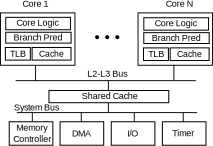
\includegraphics[width=3in]{figs/baseline.pdf}
            \caption{The timing-channel vulnerable baseline architecture.}
            \label{fig:baseline}
        \end{center}
    \end{figure}

    Figure \ref{fig:baseline} shows the baseline architecture which is later 
    extended to include timing channel protection. The architecture has 
    multiple cores, each with a branch predictor, one or more private caches, a 
    TLB, and the core logic. Each processor is connected to a shared cache 
    through an on-chip network. The multicore processor is connected to the 
    main memory and a DMA module through the system bus. 

    The hardware is concurrently shared by multiple timing compartments. As 
    shown in Figure \ref{fig:baseline}, it is possible for a timing compartment 
    to have multiple software modules which may be allocated to different 
    cores. It is also possible for timing compartments to be time multiplexd on 
    the same core (e.g.  by context switching VMs), but it is not possible for 
    timing compartments to execute concurrently on the same core (e.g. through 
    SMT).


% \section{Timing Compartments}
    Timing compartments are a new architecture primitive that control timing 
    channel leakage among software entities that share hardware. When combined 
    with explicit channel protection (such as access controls) timing 
    compartments provide total software isolation.
    A timing compartment consists of one or more software entities. Here a 
    software entitiy is some system abstraction (such as processes or threads 
    in a single OS system or virtual machines in a virtualization based system) 
    that execute software and have an owner.
    
    Timing channels between timing compartments must be controlled according to 
    a policy that meets the security requirements of the system. This policy 
    entails of a lattice of security levels such as $\mathtt{low} \leq
    \mathtt{high}$. A timing compartment can only leak information to a 
    preceeding timing compartment in the lattice. This lattice model is quite 
    expressive. The lattice $\mathtt{low} \leq \mathtt{high}$ defines a policy 
    where a high assurance software entity can not leak information to a low 
    assurance one. The lattice $\mathtt{T_1} \nleq \mathtt{T_2}, \mathtt{T_2} 
    \nleq \mathtt{T_1}$ defines a policy where $T_1$ and $T_2$ are mutually 
    distrusting. By convention, security lables share names with their timing 
    compartments. 
 
    To enforce the policy a trusted software component called the timing 
    compartment manager (TCM) confines software entities into TCs. The TCM then 
    informs the hardware of the TCs and policy. At runtime, the TCM tags 
    hardware requests with a tag to indicate the TC of the software entity that 
    made the request. 

    Timing compartments only address timing channels; they do not control 
    information flow through explicit channels. Handling these concerns 
    separately allows for more flexibility in the overall system design.  When 
    designing a secure system, implementors must consider how the cost required 
    to carry out a particular attack compares with other attacks, the potential 
    damage that could be caused by an attack, and the cost and performance 
    impact of implementing the security mechanisms needed to stop it. This 
    enables timing compartments to provide timing channel protection only to 
    software entities that need it.

    \subsection{Applications}
    This section describes how to apply timing compartments to protect the 
    vulnerable systems described in section \ref{sec:cloud_scenario}.
    \subsubsection{Cloud Computing}
    In the cloud computing system described eariler, VM1 and VM2 are both 
    running applications with high security needs. Both distrust eachother and 
    all other VMs in the system. VM3 and VM4 are running programs that require 
    a lot of performance, but have low security needs. All VMs implicitly trust 
    the hypervisor. Figure \ref{fig:cloud_tcs} shows timing compartments can be 
    applied to meet the needs of this system. VM1 and VM2 are confined to their 
    own timing compartments TC1 and TC2, but VM3 and VM4 are grouped in TC3.  
    The hypervisor is extended with a TCM and confined to TC0 since it also 
    requires timing channel protection. 
    
    \begin{figure}
        \begin{center}
            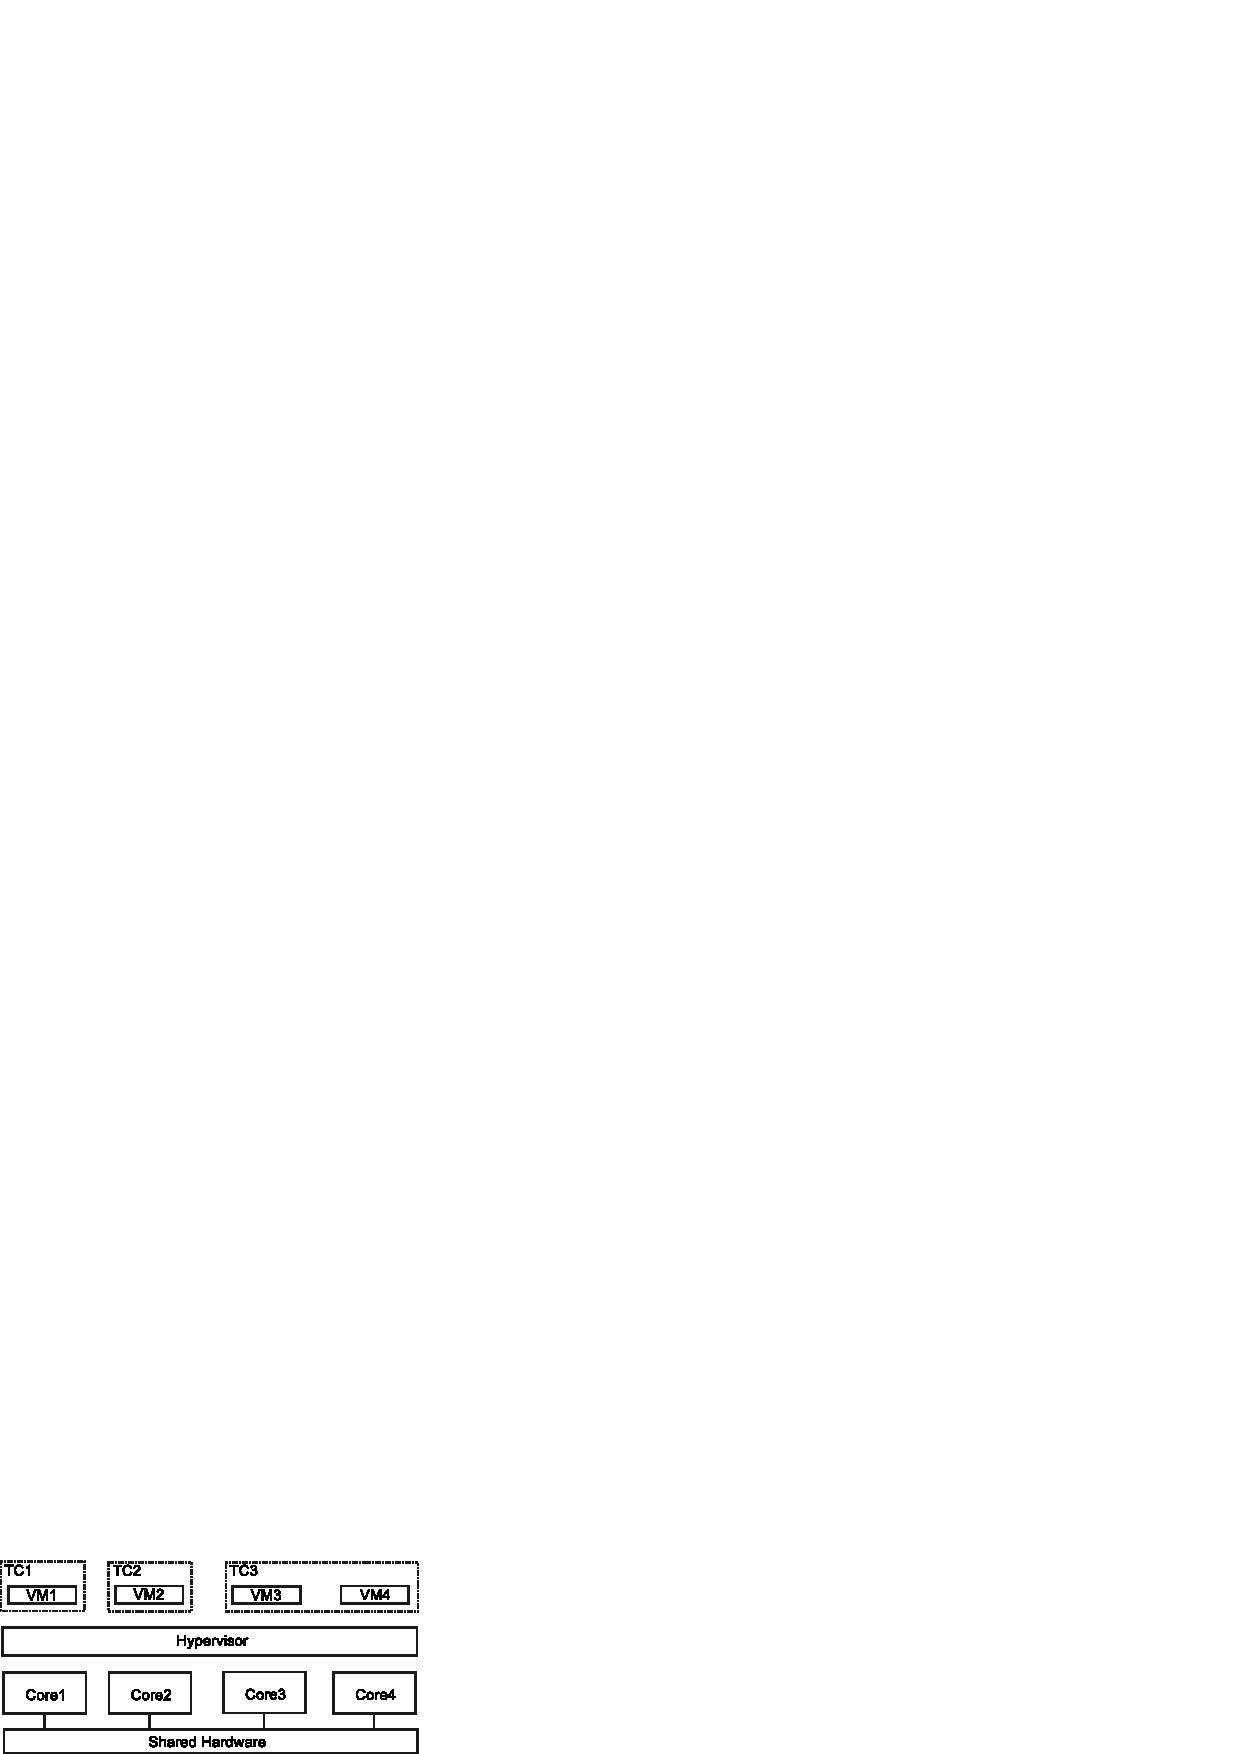
\includegraphics[width=2.1in]{figs/cloud_tcs.pdf}
            \caption{ An application of timing compartments to a cloud 
                computing environment. The hypervisor and high assurance VMs 
                are confined to their own TCs while low assurance VMs share TC3
            }
            \label{fig:cloud_tcs}
        \end{center}
    \end{figure}

    \begin{figure}
        \begin{center}
            \includegraphics[width=1.5in]{figs/cloud_lattice.pdf}
            \caption{ A lattice governing the timing compartments of the cloud 
                computing environment. TC3 preceeds TC1 and TC2. TC1 and TC2 
                are incomparable with each other, but preceed TC0
            }
            \label{fig:cloud_lattice}
        \end{center}
    \end{figure}

    The lattice in Figure \ref{fig:cloud_lattice} defines the policy. TC3 
    preceeds both TC1 and TC2 implying timing channel leakage from VM3 or VM4 
    to any other VM is not controlled. However, VM1 and VM2 cannot leak 
    information to VM3 or VM4. Additionally, VM1 and VM2 cannot leak 
    information to each other since TC1 and TC2 are incomparable. All other TCs 
    preceed TC0, so leakage from any VM to the hypervisor is not controlled, 
    but the hypervisor cannot leak any information to the VMs.This meets the 
    security requirements of VM1 and VM2 since both are totally isolated from 
    the other VMs through timing channels. Since VM3 and VM4 share a timing 
    compartment, they can share resources normally and incur minimal 
    performance overheads.

% \section{Timing Channels}
\label{sec:tc_sources}
The baseline architecture is vulnerable to microarchitectural timing channels 
caused by shared resources including the private and shared caches, the on chip 
network, the system bus, and the main memory. Furthermore, data-dependent 
variations in the timing parameters of microarchitectural components can cause 
timing channels even in the absence of sharing. In general, all 
microarchitectural timing channels may be classified as state based timing 
channels, resource contention based timing channels, or termination channels.  
We later present approaches to address timing channels of each of these kinds.

In a state based timing channel:
\begin{itemize}
    \item The time required to access a resource with state depends on the 
        contents of that state. 
    \item An adversary can observe the time required to complete requests to 
        that resource made by one security domain (that it controls).
    \item Another security domain operating on secret data can modify this 
        state, and these modifications can possibly affect the request timings 
        observable by the adversary.
    \item These modifications can possibly depend on the secret.
\end{itemize}
When all of these conditions are met, the timings that the adversary can 
observe correlate with the secret, and sensitive information may be leaked.

There is a resource contention based timing channel whenever:
\begin{itemize}
    \item A resource can concurrently service a finite number of requests and 
        this limitation can affect the time required to service a request (e.g.  
        if a request can be delayed because the resource is servicing another 
        request).
    \item An adversary can observe the time required for requests to that 
        resource made by one security domain (that it controls).
    \item Another security domain that directly operates on a secret contends 
        for the same resource and this contention can affect the timings 
        observable by the adversary.
    \item Usage of this resource by the security domain operating on the secret 
        can possibly correlate with the secret.
\end{itemize}
Together, these conditions imply that the adversary can make requests to use a 
resource with a contention based timing channel and extract secrets from these 
timings.

If instead the adversary can directly observe the time required for the 
security domain operating on a secret to complete any action (e.g. run an 
entire program or complete a memory request), this is a termination channel.  
This differs from state based and resource contention based timing channels 
wherein an adversary can only measure the timings of a security domain that it 
controls, but not the security domain directly operating on a secret. The rest 
of this section classifies the timing channel vulnerabilities due to each 
microarchitectural component into this taxonomy, and provides elucidating 
examples of these classes of timing channels.

\subsection{Private Caches}
The baseline private caches are shared among security domains whenever a core 
context switches between them. Despite the lack of concurrent sharing, private 
caches cause information leakage between context switches and through variation 
in timing not due to sharing.

Private caches impose a state based timing channel even if each security domain 
has a totally disjoint address space (i.e. no security domain can read or write 
any memory address that another security domain can read or write). Requests to 
the memory hierarchy for addresses that are stored in the cache (cache hits) 
are returned faster than requests that are not stored in the cache (cache 
misses). So, the time required to access the cache depends on its state. An 
adversary controlling a security domain can use conventional time measurement 
libraries to record cache access timings and determine which requests are hits.
The adversary controlled security domain can be context switched out for one 
that will operate on some secret. This other domain can read new memory 
addresses into the cache which may evict some of the old entries that occupied 
the cache. The memory addresses used by this domain can depend on the actual 
data of the secret, for example, through a branch condition. (In the attack 
proposed by Bernstein \cite{bernstein} the addresses read by an AES algorithm 
depend on the secret key through sboxes). Therefore, this satisfies the 
definition of a state based timing channel.

The adversary can exploit this timing channel by loading an array from memory 
that occupies as many cache lines as possible. The adversary then waits until 
the virtual machine he or she controls is context switched out and replaced 
with the security domain that will operate on the secret. This security domain 
may evict some of the cache lines of the array. When the adversarial security 
domain context switches back, the adversary can learn which cache lines were 
evicted by making requests to read each element of the array and measuring the 
timing. It will take longer to read the elements which were evicted. Unless the 
cache is fully associative, the particular cache lines that were evicted will 
depend on the addresses operated on by the victim security domain. Even if the 
cache is fully associative, the adversary can use an array that completely 
fills the cache and learn the number of cache lines read by the adversary - a 
quantity that can also depend on a secret.

Additionally, private caches also cause termination channel vulnerabilities if 
the adversary can measure the duration of an event performed by a security 
domain that operates on some secret and includes one or more private cache
accesses. In the DRM video playback usage case, an example of such an event is 
a function call in the secure world that handles a request made by the normal 
world. The adversary can measure the time between making the request (invoking
the monitor to context switch the adversarial security domain out) and being 
context switched back in. The total time required to complete the function will 
depend on the cache hit ratio which depends on program control flow and 
therefore possibly the secret. This termination channel has the interesting 
property in that it requires no interference or resource sharing between the 
two security domains at all.
 
\subsection{TLBs and Branch Predictors}
As with private caches, TLBs and branch predictors are shared among security 
domains between context switches and have state that causes the total execution 
time of tasks to correlate with private data. As a result, similar approaches 
can be taken to prevent timing channels in all three of these per-core 
resources, however, different approaches may be desirable because each resource 
affects performance differently.

\subsection{Shared Caches}
Unlike the private caches, shared caches allow concurrently executing security 
domains to interfere with one another. However, the sources of timing channels 
are still similar to those in the private cache. As with private caches, it is 
possible for an adversary to exploit the ability of a higher level security 
domain to access entries owned by a lower level domain to determine which 
addresses are used. However the lower level domain can cause interference while 
the secure domain is executing, not just between context switches. This allows 
the attacker to have finer-grained control over when interference takes place, 
potentially allowing for faster exfiltration of secrets. Similarly, if a domain 
evicts cache entries owned by another concurrently executing domain with which 
the former domain shares the cache, the latter domain can observe this and 
potentially extract secret information. As with private caches, the timing of a 
single security domain depends on it's shared cache access pattern, and 
therefore, overall timing is correlated with data values even without 
interference.

\subsection{Main Memory}
The main memory is shared between concurrently executing security domains, and 
analogous to the timing disparity between cache hits and misses, page faults in 
main memory take substantially longer than accessing entries that are present 
in main memory. So the main memory has sources of timing channels that are 
similar to the shared cache. However, the memory controller has additional 
timing channels due to resource contention. Wang et. al. classify timing 
channel sources as queueing structure interference, scheduler arbitration 
interference, and DRAM Device interference. These timing channel sources are 
summarized here.

A typical memory controller queueing structure groups memory requests by bank 
and schedules them to achieve the best performance regardless of which security 
domain the requests came from. This queueing structure interference causes the 
time that requests from one domain are scheduled to depend on the presence of 
requests from another domain. Interference can be observed whenever a request 
from one domain is chosen over a request from another, or whenever one domain 
consumes the entire capacity of the queueing structure (thereby causing 
requests from other domains to stall).

Scheduler arbitration interference causes timing channels in a conventional 
memory controller whenever requests from two different security domains for 
different banks arrive at the queue at similar times. Depending on the specific 
scheduler policy, the one request will be favored causing the other request to 
be delayed.

Lastly, contention for finite resources in the DRAM device (e.g., the command 
bus, data bus, banks, and ranks) causes interference among security domains and 
timing channels. For example, two requests to the same bank cannot be scheduled 
at the same time. If two security domains make a request for the same bank at 
the same time, one of them must be delayed.

\subsection{On Chip Network \& System Bus}

% \section{Timing Channel Protection Mechanisms}
This section proposes mechanisms that prevent all microarchitectural timing 
channels. At a high level, our approach to handling state-based timing channels 
is to apply static partitioning (or flushing where appropriate for resoureces 
that are private to a core), and our approach to handling resource contention 
based timing channels is to use time division multiplexing.  Termination 
channels are resolved by determining a worst case time for the operation and 
always returning at the worst case time. However, implementing these techniques 
for each microarchitectural component is a nuanced problem with subtle details 
that must be addressed for both efficiency and correctnes. In this section we 
discuss these techniques and show how they may be applied to each component in 
detail.

\subsection{State Based Timing Channel Protection}
\subsubsection{Static Partitioning}
The private and shared caches, TLBs, and branch predictors of each core in the 
system induce state based timing channels.  These timing channels can be 
eliminated by allocating static partitions to each security domian in the state 
of each of these resources. In states where entries may be evicted (e.g. caches 
and TLBs), a security domain may only evict entries in its own partition (and 
it may not evict entries of another partition even if the other partition has a 
lower security level).

This technique applied to the cache eliminates attacks that attempt to observe 
cache line evictions. Formerly, an adversary that controls one security domain 
could load a large array into the cache and observe which entries are evicted 
by the other domain. Now, if an adversary attempts the same attack, it will 
only be able to fill cache lines in its own domain and the other domain can 
only evict cache lines in its own domain. So, the adversary learns nothing with 
this attack. The same reasoning applies to attacks based on branch predictor 
table capacity and TLB entry eviction. For each of these microarchitectural 
timing channels, the security domain operating on a secret cannot make any 
modifications to the state that are observable by any other domain. This 
implies the state based timing channel has been eliminated.

\subsubsection{Flushing}
The private caches, TLBs, and branch predictors have the unique property that 
they are only shared among security domains between context switches. We can 
leverage this by flushing the state elements in each of these whenever  a 
context switch happens rather than statically partitioning them. This increases 
the maximum space a security domain can consume at a given time, but when a 
context switch happens there are two performance penalties. The time required 
to perform the context switch potentially increases if flushing the state 
cannot be done instantly or in parallel with other steps, and there is a 
penalty in performance due to the actual loss of state. In the private cache, 
this performance loss is a sequence of compulsory cache misses - misses that 
cannot be avoided at the beginning of execution because the cache is empty - 
that lasts until the cache is refilled with data that is useful to the current 
security domain. The TLB similarly suffers from a now empty table of address 
translations, and the branch prediction accuracy is weakened by a loss of 
history. 

Clearly there is a tradeoff between these two approaches. If context switches 
are expected to be infrequent (as may be the case if the security domains are 
not working together and the context switches are due to normal hypervisor 
management), it is likely that flushing is preferable since the performance 
loss will also be infrequent. However, if the context switches happen often (as 
in the case of the DRM processor with only a single core that context switches 
out the normal world any time the secure world must handle a request) the 
performance impact of the lost state and flush time may be more significant 
than that of the capacity lost to partitioning.

\subsubsection{Flattening}
The last technique to addressing state based timing channels eliminates the 
dependence of access time on the state by making every access take the same 
amount of time. This can be applied to a cache by treating every access as a 
cache miss. This is equivalent to eliminating the cache entirely. This has dire 
performance implications and is not likely an effective solution to address 
cache induced state based timing channels. However, this flattening technique 
is a suitable solution for the state based timing channel in the row buffer of 
the memory controller. Static partitioning cannot sensibly be applied to the 
row buffer since it contains exactly one row. Unlike caches and other state 
based timing channels, the performance lost from neglecting the caching effect 
of the row buffer is tolerable. Flattening may be applied to the row buffer by 
using a closed page row buffer management policy.

\subsection{Resource Contention Based Timing Channel Protection}
\subsubsection{Time Division Multiplexing}
This section is not yet completed, but we already know how this applies to 
memory controllers and on chip networks, so this is just a matter of writing.

\subsection{Termination Channel Protection}
Termination channels are problematic for certain usage scenarios (such as the 
DRM processor) where an adversary can observe the timing of a victim security 
domain action directly.  The private and shared caches, TLBs, branch 
predictors, and memory controller all induce termination channels whenever the 
adversary can observe the time required to complete an action that depends on a 
secret and is comprised of one or more requests to use one of these resources. 
In the DRM processor, the normal world makes requests for the secure world to 
perform some function. An adversarial normal world can measure the time it 
takes for this request to be handled, and handling the request may depend on 
any number of requests to use any of the aforementioned resources. In general, 
this timing channel can be addressed by finding a conservative upper bound on 
the action that causes the termination channel. The action must be forced to 
appear to take the worst case time on each execution. In the DRM processor 
case, this means a worst case time estimation for each secure world operation 
must be found before execution. Then whenever a secure world operation would 
normally terminate before the worst case time, it must be stalled until the 
worst case is reached.

% \section{Implementation}
\subsection{Shared Cache}
\subsection{Memory Controller}
\subsection{On Chip Network \& System Bus}
\subsection{Handling Context Switches}

% \section{Evaluation}

We evaluated the timing compartments architecture using the gem5 architectural 
simulator~\cite{gem5} integrated with the DRAMSim2~\cite{DRAMSim2} 
memory simulator. Our experiments use multiprogram workloads 
comprised of SPEC2006 benchmarks compiled for the ARM ISA. 

Table~\ref{tab:config} shows our system configuration.
The cores use the gem5 ``O3`` out-of-order core model which runs at 2GHz. 
Each core has private 32KB L1 instruction and data caches, and private 256KB L2 
cache. The cores share a 4MB L3 cache. We derived cache configuration 
parameters from the Intel Xeon E3-1220L, which is a two core architecture used 
by Amazon EC2. In DRAMSim2, we simulate a 667MHz 2GB DDR3 memory. The 
interconnects in the simulator runs at 1GHz. Unless specified otherwise, each experiment is 
fastforwarded for 1 billion instructions, and run for 100 million 
instructions. We will first describe our security evaluation and then show
the performance evaluation.

\begin{table}
    \caption{Simulator configuration parameters.}
    \centering
    \begin{tabular}{|l|l|l|r|}
        \hline
        \multicolumn{3}{|l|}{gem5 core model} & ``O3''        \\\hline
        \multicolumn{3}{|l|}{CPU Clock}    & 2GHz             \\\hline
        \hline
        \multicolumn{2}{|l|}{Memory}             & 2GB    & 667MHz  \\\hline
        \hline
        \multicolumn{3}{|l|}{Network Clock}      & 1GHz \\\hline
        \hline
        L1d / L1i  & 32kB   & 2-way  & 2 cycles\\\hline
        L2         & 256kB  & 8-way  & 7 cycles \\\hline
        L3         & 4MB    & 16-way & 17 cycles  \\\hline
    \end{tabular}
    \label{tab:config}
\end{table}

\subsection{Security Evaluation}

To experimentally evaluate the security of the timing channel protection in our 
architecture, we use a two-core system with two timing compartments, TC0 and
TC1, running concurrently. The protection policy is configured to disallow any 
timing channels between the two compartments. If the number of cycles required 
to execute a certain number of instructions for a particular benchmark running on 
TC0 depends on which benchmark is running on TC1, it indicates timing 
interference exists that can be exploited to leak information about TC0. A 
secure system should guarantee the benchmark running in TC0 always uses the 
same number of cycles to finish regardless of which benchmark TC1 is running. 

Using the rule above, we evaluated the security of our architecture by running 
a fixed benchmark on TC0 while varying the benchmark on TC1. Then we compared 
the total execution time for the fixed benchmark in different runs. We 
evaluated our architecture as well as the baseline insecure architecture which 
does not implement any protection. As expected, the results for the baseline 
show the execution time of a particular benchmark on Core 0 changes significantly 
depending on the benchmark on Core 1, indicating timing channels exist between
the two cores. On the other hand, when running each pair of benchmarks with 
timing channel protection we observed no execution time difference by changing 
which program runs concurrently with TC0.

\subsection{Time Slice Coordination}
\label{sec:eval_coord}
We analyzed the L2 miss path TDM scheduling problem using our own simulator.
Given the turn lengths and offsets of each device, the latency of a request can be 
determined based on the cycle in which a request arrives in the schedule.
Since a schedule repeats after the least common multiple of each 
turn length in the schedule multiplied by the number of timing compartments, 
each possible latency for a schedule can be enumerated. The simulator finds
each possible latency in a schedule, and calculates the 
expected value of this latency assuming the arrival time at the L2-L3 bus is 
uniform random.

Using this simulator, we exhaustively searched for the optimal L3 hit path 
schedule with the parameters summarized in table ~\ref{tab:coord_param}. The 
search space includes turn lengths from 1-25 cycles and all possible offsets 
for each turn length. We confirmed that the intuitive schedule described in 
Section \ref{sec:coordination} achieves the highest expected value of the 
latencies for L2 misses that hit in the L3.
Fixing the turn lengths to the optimal ones and adjusting only the offsets,
the worst case latency is 19.6\% worse than the optimal schedule, showing
that coordinating the hit path is important.

\begin{table}
    \caption{Time slice coordination simulator paramaters}
    \centering
    \begin{tabular}{|r|r|}
        \hline
        $t_{req}$  &   1 cycle \\\hline
        $t_{resp}$ & 9 cycles \\\hline
        $t_{L3}$   &   9 cycles \\\hline
        $t_{read}$ & 36 cycles \\\hline
    \end{tabular}
    \label{tab:l2_miss_schedules}
\end{table}

The search space for schedules involving every resource in the L2 miss path
is far too large to search exhaustively.
Instead we used integer linear programming optimization 
techniques. Changing a turn length or offset slightly can drastically affect 
the performance, so the search space has many relative minima. We used 
our own simulated annealing optimizer to avoid getting stuck at relative minima 
and increase our chances of finding a global minimum.

We used the optimizer to 
study the latency of L2 misses that miss in the L3.
After initializing the optimizer with the L3 miss schedule summarized in 
Figure~\ref{fig:miss_schedules}, the optimizer did not find a 
better schedule after 20,000 iterations. Fixing the turn lengths to be the same 
as the best schedule found and sweeping only the space of offsets,
the worst-case schedule performed 2.38X
worse than the optimal schedule.

We used the same optimizer to study the latency of L2 misses in general 
assuming a 90\% L3 cache hit rate.
Optimizing for the L2 miss rate overall is a harder problem since it requires a balance 
bewtween the best L3 miss case and L3 hit case parameters. The 
schedule produced by the optimizer was not one that made any intuitive sense. 
However, the optimal schedule was 8.67X better than the worst schedule that 
used the same turn lengths as the best schedule (and changed only the offsets).

The results for schedule selection study are summarized in Table 
\ref{tab:coord_results}. Overall, scheduling 
interdependent time multiplexed devices is a challenging problem, but the gap 
between the worst and optimal cases show that it is important.

\begin{table}
    \caption{Scheduling Selection Study Results.}
    \centering
    \begin{tabular}{|l|l|l|l|}
        \hline
        \multicolumn{1}{|l|}{Optimized Quantity} & Search & Min & Max \\\hline
        \multicolumn{1}{|l|}{L3 Hit Latency} & Exhaustive & 25.5 & 30.5 \\\hline
        \multicolumn{1}{|l|}{L3 Miss Latency} & Simulated Annealing& 139.5 & 334.5 \\\hline
        \multicolumn{1}{|l|}{L2 Miss Latency} & Simulated Annealing& 38.6 & 344.5 \\\hline
    \end{tabular}
    \label{tab:coord_results}
\end{table}

\subsection{Performance Evaluation}

The timing compartment architecture extends the insecure baseline with
static partitioning and time multiplexing to secure the shared hardware 
resources. These changes lead to underutilization, and thus, a performance
overhead. To evaluate the performance overhead, we ran pairs of
SPEC2006 benchmarks, and measured the execution time of the benchmark
in TC0. Since the timing channel protection mechanisms primarily affect the memory 
hierarchy, the memory intensity of the benchmarks is related to the performance 
overhead.
The memory intensity of each benchmark, in memory requests per thousand 
instructions, during the program segment used for our experiments is shown in
Figure~\ref{fig:memstudy}. Of the SPEC2006 benchmarks, mcf has the most memory 
requests, while astar has none after fast-forwarding for 1B instructions.

For the baseline architecture, we calculate the average execution time of the 
benchmark on Core 0 by averaging among runs with different benchmarks on Core 1. 
The execution time of the benchmark in Core 0 is impacted by the benchmark in 
Core 1. In the timing compartments architecture, the execution time of TC0 (on 
Core 0) is independent of workloads running in other timing compartments.

\begin{figure}
    \begin{center}
        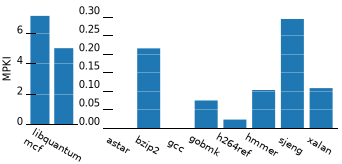
\includegraphics[width=3.4in]{figs/mpki_merged.pdf}
        \caption{Memory intensity of SPEC2006 benchmarks.}
        \label{fig:memstudy}
    \end{center}
\end{figure}

Figure~\ref{fig:performance} shows the performance overhead of full system 
protection as well as the overhead incurred by the changes to the memory 
controller (mc), the cache (waypart), the L3 to memory bus (membus), and the L2 
to L3 bus (L2L3) individually compared to the insecure baseline. The
overheads for libquantum and mcf, which are particularly memory intensive, are 
highest at 69\% and 18\% respectively. However, the arithmetic mean of the 
total overhead is quite low at roughly 9\%. Memory controller protection incurs 
by far the most overhead suggesting the impact on memory bandwidth is more 
significant than bus or cache underutilization. Overall, the results show that 
the timing compartments are viable for applications that require high assurance 
for software isolation.

\begin{figure}
    \begin{center}
        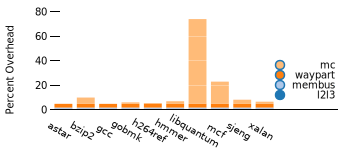
\includegraphics[width=3.4in]{figs/breakdown.pdf}
        \caption{Performance overhead for 2 TCs.}
        \label{fig:performance}
    \end{center}
\end{figure}

The performance overhead is likely to increase as the number of timing 
compartment scales up. To study the impact of the number of timing 
compartments, we evaluated the performance overhead with three and four timing 
compartments on a 4-core  processor, each occupying one core and private L1 and 
L2 caches. They share a 4MB L3 cache. We do not evaluate all permutations of 4 
benchmarks. Instead, we only evaluate the subset of these permutations where 
TC1, TC2, and TC3 are executing the same benchmark. As before, each of these 
workloads with the same program in TC0 is averaged.

The performance overhead as the number of timing compartments increases is 
shown in Figure~\ref{fig:scalability}. The arithmetic mean of the overheads for 
each benchmark for 2, 3 and 4 timing compartments are 9\%, 17\%, and 24\% 
respectively. For libquantum which is particularly memory intensive, the 
overheads are 76\%, 140\%, and 184\% for 2, 3, and 4 timing compartments. The 
results suggest that the overhead of timing timing channel protection is rather 
insensitive to the number of timing compartments for compute-bound 
applications. For memory-intensive applications, the overhead can increase 
noticeably. However, the results still suggest that timing compartments can 
allow distrusting software entities to share hardware and provide better 
overall performance than running them on separate dedicated machines.

\begin{figure}
    \begin{center}
        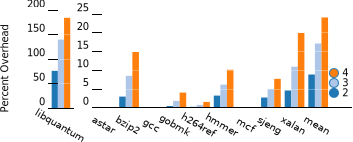
\includegraphics[width=3.4in]{figs/scalability_split.pdf}
        \caption{Performance overhead for 4 TCs.}
        \label{fig:scalability}
    \end{center}
\end{figure}

While future multi-core systems are likely to have a large number of processing 
cores, we note that many security applications will not require many timing 
compartments to be used concurrently. For example, the BYOD application only 
requires two TCs no matter how many cores exist in the system. Similarly, in 
a high-assurance cloud computing environment, the cloud provider can limit the
number of high-assurance virtual machines that can be located on each physical
system while increasing the system utilization by co-locating non-secure
virtual machines with high-assurance ones.

\subsection{Cache Coherence Performance Overhead}
Adding the timing channel protection for snooping bus can introduce some performance overhead. We evaluate some 
splash2~\cite{splash2} benchmarks in gem5. The system we model is the one shown in Figure~\ref{fig:coherent_system}.
We use the same splash2 benchmarks for Attacker0 and Attacker1, each consists of two threads. We terminate the simulation
when thread on core 0 reaches 100M instructions. 
Our baseline is a system where every other timing channel protection scheme we proposed is implemented except for the snooping bus.
We then compare it with the system where the snooping bus is also protected. This comparison enables us to quantify the exact overhead introduced by adding cache coherence protection. 

The results are shown in Figure~\ref{fig:splash2}. As can be seen, the overhead of adding cache coherence protection is
quite low, with the highest overhead less than 1.5\%. In some cases the protection scheme even outperform the baseline, 
mainly because the round-robin scheduling may have avoided some snooping bus contention in the baseline scheduling. 
The main reason for the low overhead is that the coherent traffic is quite rare in programs, hence the round-robin
snooping bus will not cause much overhead to the overall program execution time.

\begin{figure}
    \begin{center}
        \includegraphics[width=2.79in]{figs/splash2.pdf}
        \caption{Performance Overhead of Cache Coherence Protection}
        \label{fig:splash2}
    \end{center}
\end{figure}

% \section{Related Work}

Previous studies identified 
a number of microarchitectural timing channels 
caches~\cite{percival,bernstein,caseofaes,remoteaes,analyticalcache,collision,
deconstructing,cachegames}, branch predictors 
\cite{branchpred,predictingbranch}, processor
pipelines \cite{pipelines}, networks on chip~\cite{yaonocs,surfnoc}, and memory
controllers~\cite{ushpca14,fletcher-hpca14}. 
Also, people have proposed solutions for timing channels in
individual components such as caches~\cite{newcache,deconstructing}, memory
controllers~\cite{ushpca14,fletcher-hpca14}, and on-chip network
~\cite{yaonocs,surfnoc}.
However, the previous work has
so far focused on individual component. This work represents the first attempt
at designing a full microprocessor with complete internal timing channel protection.
Our integration efforts also exposed new sources of timing channels in module
interfaces such as MSHRs and cache/memory response ports.

%However, this paper presents the first microarchitecture to address all 
%internal microarchitectural timing channels. 

Ascend~\cite{ascend} proposes a
microarchitecture that aims to eliminate external timing channels so that
even untrusted software can execute without leaking any confidential
data. This presents a powerful option if physical attacks need to be
considered. However, Ascend does not allow a processor to be shared by
multiple software components at the same time, and does not address 
any internal timing channels.
Execution leases~\cite{execution_leases} 
provide another external timing channel solution at the hardware level by 
enforcing strict upper bounds on the execution times of program subsections. 

Timing channels are a form of information flow, and there is a large body
of work on information flow control. For example, language-level approaches
track information flow that is visible at the program level to either 
eliminate~\cite{quantleaks} or 
reduce~\cite{mitigation1,mitigation2,mitigation3} timing channels. 
However, language-level approaches cannot fully control microarchitecture-level
timing channels because traditional instruction set architecture hides
timing inside a processor.
At the 
systems level, information flow control has been used to control
explicit communication channels~\cite{flume-sosp07,histar-sosp06,laminar-pldi09}. 
These software approaches can control explicit information flows or external
timing channels that the timing compartments do not handle.
The timing compartments complement these software approach by
controlling microarchitectural timing channels.

There have been recent efforts on verifying information flow properties
of hardware including certain timing channels. For example, GLIFT
\cite{glift-asplos09} dynamically tracks all information flows, including timing channels,
at the logic gate level. 
The idea in GLIFT has been extended to develop verifying
information flow properties using gate-level simulations
\cite{glift-dac10,glift-dac11,glift-isca11} and a 
hardware description language
~\cite{caisson-plas10,caisson-pldi11,sapper-plas13}.
However, these approaches so far have only been applied to simple
processors and a very strict isolation mechanism. 
This paper studies timing channel protection on complex multi-core processors.


% \section{Conclusion}
This paper presents timing compartments, which provide an architecture 
abstraction to eliminate timing channels. When used in conjunction with access 
controls, timing compartments can provide total software-level isolation since 
other side or covert channel attacks require physical access. To realize 
timing compartments, we designed a full multiprocessor microarchitecture 
that eliminates all inter-program timing channels and evaluated it in the gem5 
architectural simulator. Our results show that the overheads are low.


%\bstctlcite{bstctl:etal, bstctl:nodash, bstctl:simpurl}
%\bibliographystyle{IEEEtranS}
 \bibliographystyle{abbrv}
%\bibliographystyle{latex8}
 \bibliography{paper}

\end{document}
